\chapter{氧疗与人工气道管理}

\section{前沿学术综述}

\subsubsection{氧气疗法}

氧气是机体组织细胞能量代谢所必需的物质。必须有充足的氧气,细胞才能维持其生理功能。机体对氧气的生理需求和缺氧对机体的危害,使临床医师充分认识到氧气的重要性,特别是在危重患者的救治中,氧疗具有重要的治疗作用。

(1)氧疗的目的

纠正低氧血症:增加吸入氧浓度,提高肺泡氧分压,可不同程度地纠正低张性低氧血症。正常情况下,从大气到组织细胞各个水平的氧分压值见图\ref{fig9-1},20mmHg为细胞无氧代谢阈值,氧分压<20mmHg,组织细胞即开始无氧代谢。纠正低氧血症对防止组织缺氧具有重要意义。

\begin{figure}[!htbp]
 \centering
 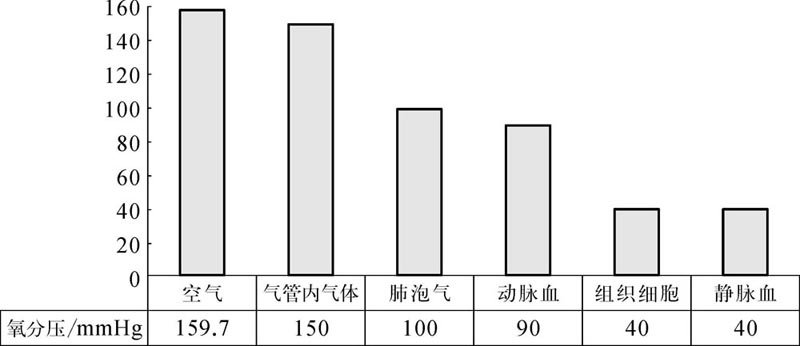
\includegraphics{./images/Image00069.jpg}
 \captionsetup{justification=centering}
 \caption{从大气到组织细胞各个水平的氧分压值梯度}
 \label{fig9-1}
  \end{figure} 

降低呼吸功:低氧血症和缺氧及其引起的酸中毒刺激呼吸中枢,作为代偿性反应,呼吸频率加快、通气量增加,引起呼吸肌做功增加,结果呼吸氧耗增加,可能形成恶性循环,导致低氧血症加重。提高吸入氧浓度,可降低机体对通气的需要,从而降低呼吸功。

减少心肌做功:低氧血症或缺氧可引起心血管系统发生代偿性反应,使心率增快、心输出量增加、外周血管收缩、血压升高,其结果是心肌做功增加,心肌氧耗增加,可能加重心肌的氧供和氧需的失衡。提高吸入氧浓度,可纠正低氧血症,缓解心血管系统的代偿性反应,减少心肌做功。

(2)氧疗的装置 根据氧疗系统提供的气体是否能够满足患者吸气的需要,一般将氧疗装置分为高流量系统和低流量系统。值得注意的是,高流量与低流量并不等同于高浓度与低浓度吸氧。不同氧疗装置氧流量与吸入氧浓度之间的关系不同。

(3)氧疗效果的评价 氧疗的目的不仅在于纠正低氧血症,更为重要的是维持心血管系统和呼吸系统的功能,保证组织器官足够的氧供。氧疗实际上是纠正组织缺氧的重要手段之一。因此,对氧疗的评价不仅包括对器官功能进行评估,而且也应包括器官组织氧代谢的评估。

(4)氧疗的副作用 氧疗在临床治疗中有重要作用,但临床医师对氧气的毒性普遍认识不足。氧气实际上也是一种“药物”,不但应注意其使用剂量,还应注意其毒副作用。氧疗的毒副作用主要与高浓度吸入有关,其中最主要的副作用有去氮性肺不张和氧中毒。

\subsubsection{人工气道的建立和管理}

人工气道是为了保证气道通畅而在生理气道与其他气源之间建立的连接,分为上人工气道和下人工气道,是危重症患者常用的抢救措施之一。上人工气道包括口咽气道和鼻咽气道,下人工气道包括气管插管和气管切开等。

建立人工气道的目的是保持患者气道的通畅,有助于呼吸道分泌物的清除及进行机械通气。人工气道的应用指征取决于患者呼吸、循环和神经系统功能状况。结合患者的病情及治疗需要选择适当的人工气道。

人工气道的建立使患者上呼吸道功能丧失,而继发感染、气管导管意外脱出或梗阻等又会加重病情,甚至危及生命。如果气道管理仅作为一项医生和护士分开训练和管理的普通技术,就容易造成医生忽视人工气管建立后的气道管理;护士往往被动配合医生完成人工气道的建立,缺乏主动判断和实施意识;医护之间缺乏沟通而没有及时预见性地评估气道状况,将致错过关键的处理时机。规范的气道管理可减少人工气道并发症。由此可见,气道管理是维系生命最重要的措施之一,体现了重症医学科的救治和管理水平。

2004年加拿大危重病学会和危重病临床试验组联合专家委员会,以及2005年美国胸科学会和感染疾病学会,先后基于循证医学证据制定了院内获得性肺炎及呼吸机相关性肺炎方面的指南
\protect\hyperlink{text00015.htmlux5cux23ch1-14}{\textsuperscript{{[}1{]}}}
\textsuperscript{,}
\protect\hyperlink{text00015.htmlux5cux23ch2-14}{\textsuperscript{{[}2{]}}}
,针对人工气道管理和非抗生素预防策略方面提出了指导性意见。而近年来关于建立人工气道的方式及时机的选择、气管导管声门下潴留物的引流和气道湿化等相关方面又有新的研究,为临床治疗的具体实施提供了更多的依据。

气管插管和气管切开是临床上常用的建立人工气道方法。在循环严重不稳定的情况下,即使动脉氧合尚能维持也应早期开放气道进行有创机械通气,纠正组织缺氧。当然,在紧急开放气道时更应关注是否存在困难插管。

1985年经皮扩张气管切开术首次应用于临床,随着科技的发展,切开技术和器材在不断改进,近年来在国内广泛应用,并出现了许多改良技术。在气管切开方式的选择方面,经皮扩张气管切开术相对于传统的直视下气管切开术,显示出一定优势,可缩短手术操作时间和减少气管切开的并发症,并可能减少重症医学科住院时间和医疗费用
\protect\hyperlink{text00015.htmlux5cux23ch3-14}{\textsuperscript{{[}3{]}}}
。随着医疗技术的发展,经皮扩张气管切开已被应用于急诊创伤、凝血功能障碍的患者
\protect\hyperlink{text00015.htmlux5cux23ch4-14}{\textsuperscript{{[}4{]}}}
\textsuperscript{~}
\protect\hyperlink{text00015.htmlux5cux23ch6-14}{\textsuperscript{{[}6{]}}}
。对于需要长期机械通气或保留人工气道的患者,研究表明早期气管切开(平均机械通气时间为7天),可降低机械通气时间和重症医学科住院时间,但不降低呼吸机相关性肺炎发生率和病死率
\protect\hyperlink{text00015.htmlux5cux23ch7-14}{\textsuperscript{{[}7{]}}}
\textsuperscript{,}
\protect\hyperlink{text00015.htmlux5cux23ch8-14}{\textsuperscript{{[}8{]}}}
。

在人工气道管理方面,应维持合适的气囊压力(气囊压力一般维持在25~35cm
H\textsubscript{2}
O),可以通过气囊压力测定仪测定,或通过寻找最小封闭压力和最小封闭容积调整气囊压力,有效的声门下吸引可减少误吸,防止呼吸机相关性肺炎。研究显示,持续声门下吸引可以延缓呼吸机相关性肺炎的发生,降低呼吸机相关性肺炎的发生率,且能明显降低费用
\protect\hyperlink{text00015.htmlux5cux23ch9-14}{\textsuperscript{{[}9{]}}}
。

对于危重病患者,尤其建立人工气道者,合适的气道局部湿化非常重要,这在输液量严格控制的患者中尤为必要。近年来,新型的湿热交换器、附加电加热丝管路加热的湿化器逐渐运用于临床。相对于加温湿化器,湿热交换器操作方便,有利于感染控制,减少管路细菌的定植,但在降低呼吸机相关性肺炎发生率方面尚无明确的证据
\protect\hyperlink{text00015.htmlux5cux23ch10-14}{\textsuperscript{{[}10{]}}}
\textsuperscript{,}
\protect\hyperlink{text00015.htmlux5cux23ch11-14}{\textsuperscript{{[}11{]}}}
。

\section{临床问题}

\subsection{氧气疗法}

\subsubsection{为什么说氧气是一种药物?}

氧气应用于临床患者治疗已有一个半世纪,但直到1945年,有关氧气的生理作用仍然有争议。氧气是机体组织细胞能量代谢所必需的物质。必须有充足的氧气,细胞才能维持其生理功能。机体对氧气的生理需求和缺氧对机体的危害,使临床医师充分认识到氧气的重要性。但临床医师对氧气的毒性却普遍认识不足。由于高氧环境往往产生高浓度的氧自由基,长时间吸入高浓度氧气,可引起非心源性肺水肿,即急性呼吸窘迫综合征(ARDS)。新生儿吸入高浓度氧,除引起ARDS外,还可能引起视网膜病变及晶状体纤维增殖症,导致失明。无疑,长时间吸入高浓度氧对机体是有害的。

另外,吸入氧浓度的调整也是非常重要的。慢性阻塞性肺疾病急性加重期的患者,如吸入氧浓度过高,可引起呼吸中枢抑制,一般要求吸入氧浓度不宜高于30%或35%(氧流量不超过3L/分钟)。对于换气功能障碍的患者,如急性呼吸窘迫综合征,必须根据缺氧的程度,调整吸入氧浓度。

氧气实际上就是一种“药物”,临床应用时不但应注意其使用剂量,还应注意其毒副作用。

\subsubsection{氧疗的高流量系统与低流量系统有什么不同?}

根据氧疗系统提供的气体是否能够满足患者吸气的需要,一般将氧疗装置分为高流量和低流量系统。值得注意的是,高流量与低流量并不等同于高浓度和低浓度吸氧。

高流量系统提供的气流能够满足吸气的需要,患者不需额外吸入空气。该系统提供较高的气体流速及足够大的贮气囊,气体量能够完全满足患者吸气所需。须特别注意的是,高流量系统实施氧疗并不意味着吸入气氧浓度较高,高流量系统可提供氧浓度较高的气体,亦可提供较氧浓度较低的气体,该系统的主要优点为:①能够提供较准确的、不同氧浓度的气体,而且氧浓度不受患者呼吸模式的影响;②气流完全由系统提供,可根据患者需要调整气体的温度和湿度。

多数高流量系统采用带有Venturi装置的面罩,该装置利用Beroulli原理,氧气通过一较狭窄的喷头高速喷出,高速气流的周围形成负压,导致空气卷入主气流中,使系统气流量明显增加。采用Venturi装置的高流量系统,喷头的大小和空气卷入孔的大小决定吸入气的氧浓度,而氧流速则决定了该系统所能提供的气体量。高流量系统提供的气流速应超过患者峰值流速,而且提供的气体量应当是患者通气量的4倍以上。

低流量系统提供的气流不能完全满足患者吸气的需要,需额外吸入部分空气。该系统可提供的气体氧浓度为21%~90%。吸入氧浓度由以下因素决定:①贮气囊的大小;②氧流量;③患者的呼吸模式(潮气量、呼吸频率及吸气时间等)。

低流量系统提供的气体氧浓度不很准确,但患者更为舒适,应用较为方便,而且比较经济。常用的低流量系统包括鼻塞、鼻导管、普通面罩、带有贮气囊的面罩等。低流量系统实施氧疗时,吸入氧浓度一般低于60%,要进一步提高吸入氧浓度,需应用带有贮气囊的面罩。

\subsubsection{不同的氧疗系统提供的吸入氧浓度有何不同?}

高或低流量氧疗系统氧流量与吸入氧浓度之间的关系不同,见表\ref{tab9-1}。\footnote{* 括号内数值为进入Venturi面罩的空气流量。表中吸入氧浓度仅供参考。}

\begin{table}[htbp]
\centering
\caption{氧流量与吸入氧浓度之间的关系}
\label{tab9-1}
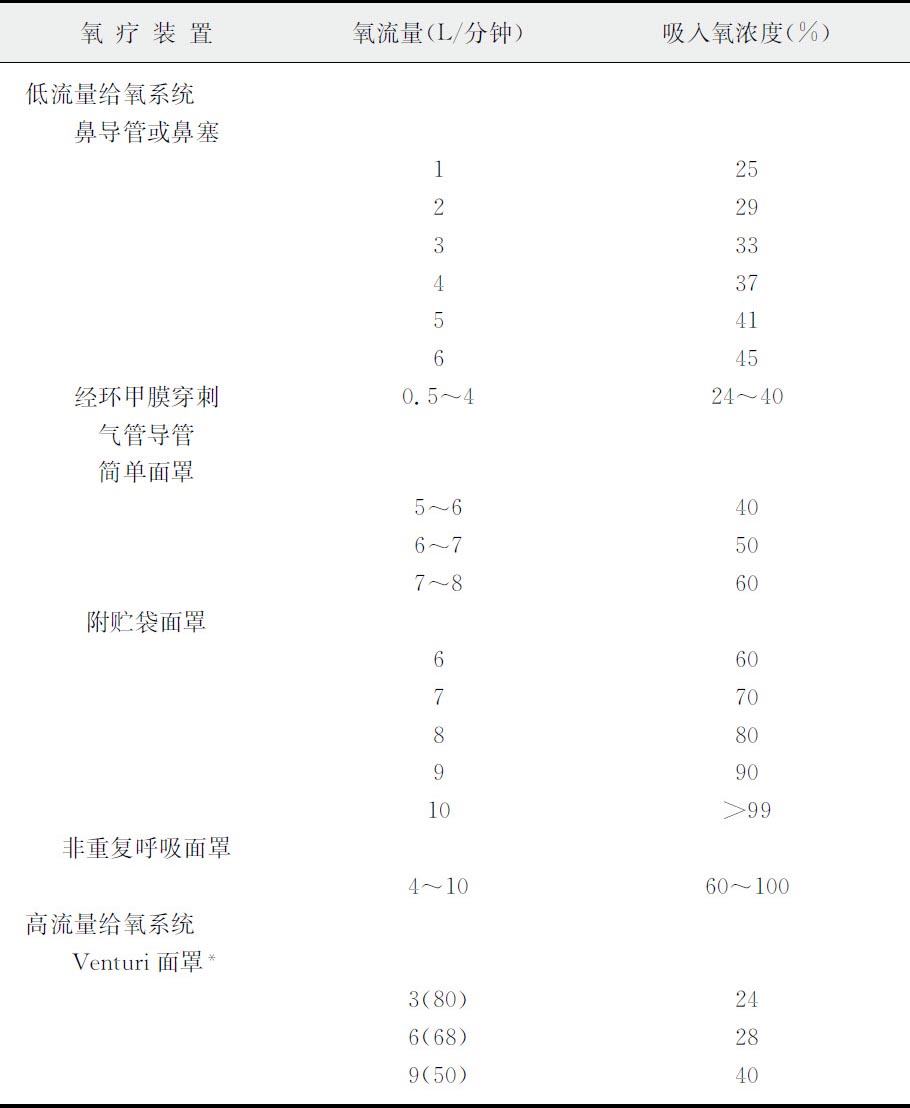
\includegraphics[width=\textwidth,height=\textheight,keepaspectratio]{./images/Image00070.jpg}
\end{table}



\subsubsection{采用低流量或高流量氧疗系统的指征是什么?}

当患者有指征接受氧疗时,应确定采用何种氧疗系统。低流量和高流量系统各有利弊。与高流量系统比较,低流量系统具有以下优点:①患者易于耐受,较为舒适;②实施较方便。但低流量系统的缺点也很明显:①低流量系统的气体不能满足患者吸气的需要,需额外吸入空气,使吸入氧浓度不稳定;②吸入氧浓度受患者呼吸模式的影响较大。高流量系统提供的气体氧浓度较为稳定,基本不受患者呼吸模式的影响。总的来说,对于病情稳定、呼吸平稳,而且对吸入氧浓度的准确性要求不高的患者,宜采用低流量氧疗系统,反之,应采用高流量氧疗系统。

一般认为,采用低流量氧疗系统应具备以下指征:①潮气量300~700ml;②呼吸频率低于25次/分钟;③呼吸规则而稳定。不符合上述任一条件的患者,均应采用高流量系统。一般来说,需接受氧疗的患者中,绝大多数患者(大约75%)只需采取低流量系统,即可达到氧疗的目标。

经过积极的氧疗措施不能奏效时,应早期气管插管,采用机械通气治疗。

\subsubsection{鼻导管吸氧时,氧流量是否是决定吸入氧浓度的唯一因素?}

采用鼻导管或鼻塞氧疗时,一般认为吸入氧浓度与吸入氧流量大致有如下关系:吸入氧浓度=21+4×吸入氧流量(L/分钟)。实际上,吸入氧浓度还受潮气量和呼吸频率的影响------张口呼吸、说话、咳嗽和进食时,即使氧流量不变,吸入氧浓度也会降低。

下面以“正常人”以“正常呼吸模式”进行呼吸为例做一简要说明:

\begin{center}
\begin{tabular}{ll}
  参数&参考值\\
  潮气量&500ml\\
  呼吸频率&20次/分\\
  吸气时间&1秒\\
  呼气时间&2秒\\
  口鼻咽解剖死腔&50ml
\end{tabular}
\end{center}



鼻导管吸氧流量为6L/分钟(100ml/秒)。假定呼气在呼气时间的前1.5秒(75%)完成,则最后的0.5秒几乎无气体呼出,来自鼻导管的纯氧(吸氧流量为6L/分钟,即100ml/秒)将在这0.5秒中将口鼻咽解剖死腔充满。那么,在1秒的吸气时间内,吸气潮气量由3个部分组成:①来自口鼻咽解剖死腔的50ml纯氧;②来自鼻导管的100ml纯氧,即100ml/秒×1秒;③500ml潮气量中,需吸入350ml的空气(氧浓度为20%左右),则氧气为350ml×20%=70ml。

可见,500ml吸气潮气量中含有220ml的纯氧(50ml+100ml+70ml),则吸入氧浓度为44%(220ml/500ml)。也就是说在“理想通气状态下”,通过鼻导管吸入流量为6L/分钟的氧气时,其吸入氧浓度为44%。

在其他条件不变的情况下,若将氧流量从1L/分钟逐渐增加至6L/分钟,则氧流量每变化1L/分钟,吸入氧浓度大约相应变化4%。这就是上述氧流量与吸入氧浓度关系方程的推算依据。

对于同一患者,其他条件不变,仅潮气量减少1/2,即250ml,则吸气潮气量的构成将发生明显变化:①来自口鼻咽解剖死腔的50ml纯氧;②来自鼻导管的100ml纯氧,即100ml/秒×1秒;③250ml潮气量中,需吸入100ml的空气(氧浓度为20%左右),则氧气为100ml×20%=20ml。

可见,250ml吸气潮气量中含有170ml的纯氧(50ml+100ml+20ml),则吸入氧浓度为68%(170ml/250ml)。因此,潮气量越大或呼吸频率越快,吸入氧浓度越低;反之,潮气量越小或呼吸频率越慢,吸入氧浓度越高(↑潮气量→吸入氧浓度↓;↓潮气量→吸入氧浓度↑)。

只要通气模式不发生变化,鼻导管或鼻塞可提供相对稳定的吸入氧浓度。但是认为鼻导管或鼻塞可确保稳定的低浓度氧疗则是错误的。

另外,应用鼻导管或鼻塞时,氧流量不应超过6L/分钟。这与鼻咽部解剖死腔已被氧气完全预充有关,提高氧流量不可能进一步增加吸入氧浓度,此时要提高吸入氧浓度,须加用氧贮气囊。

\subsubsection{如何使用普通面罩实施氧疗?}

普通面罩一般用塑料或硅胶制成,重量较轻,无单向活瓣或贮气袋,呼出气通过面罩上的小孔排出。面罩需紧贴口鼻周围,用绑带固定于头枕部。即使氧气供应暂时中止,空气仍可从面罩上的小孔和面罩周围的缝隙流入。另外,系统可提供较好的湿化。但普通面罩影响患者的进食和说话,睡眠变换体位或烦躁不安时易脱落或移位,患者呕吐时易发生呕吐物误吸。

面罩死腔及其“贮袋效应”影响了氧流量和吸入氧浓度之间的关系。氧流量需在5~6L/分钟以上,才可将面罩内的呼出气(包括二氧化碳)冲洗排出,最大吸入氧浓度为50%~60%。氧流量>8L/分钟时,吸入氧浓度不会进一步增加。如氧流量过低,不仅吸入氧浓度下降,而且呼出气的二氧化碳可在面罩内积聚,导致二氧化碳重复吸入。患者通气模式改变同样会影响吸入氧浓度。潮气量越大或吸气流速越快,氧气被空气稀释越多,吸入氧浓度越低;在一定范围内,氧流量越大,吸入氧浓度越高。呼吸缓慢的患者,采用普通面罩可获得较高的吸入氧浓度,而呼吸频速的患者则吸入氧浓度较低。所以,普通面罩不宜用于呼吸频速和严重低氧血症的慢性阻塞性肺疾病并发急性通气功能障碍或急性限制性疾病的患者(如急性肺水肿)。

\subsubsection{部分重复呼吸面罩与无重复呼吸面罩有什么区别?}

未行气管切开或气管插管的患者需吸入高浓度氧气(吸入氧浓度>60%)时,需在普通面罩上加装一体积600~1000ml的储气袋。氧流量须在5L/分钟以上,以确保储气袋适当充盈和将面罩内二氧化碳冲洗出。面罩和储气袋间无单向活瓣为部分重复呼吸面罩,有单向活瓣则为无重复呼吸面罩。应用附有储袋面罩的目的是提供较高吸入氧浓度。根据呼出气体的重复吸入程度可将氧疗系统分为以下两种:

(1)部分重复呼吸面罩(图\ref{fig9-2}) 该装置允许患者重复吸入部分呼出气体,以减少氧气消耗。氧气从面罩的颈部流入,在吸气相直接进入面罩,而在呼气相则进入储气袋。理想情况下,患者呼气时,呼出气的前1/3进入储气袋,与储气袋中的纯氧混合。呼出气的前1/3主要来自解剖死腔。此部分气体在使用部分重复呼吸面罩后不久,氧浓度较高。当储气袋被纯氧和呼出气的前1/3充满后,其内部压力迫使呼出气的后2/3(包括二氧化碳负荷)从呼气孔排出。在密封较好的部分重复呼吸面罩,氧流量为6~10L/分钟时,吸入氧浓度可达35%~60%。

\begin{figure}[!htbp]
 \centering
 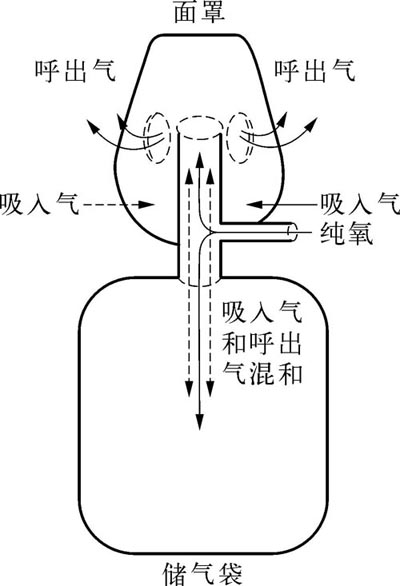
\includegraphics{./images/Image00072.jpg}
 \captionsetup{justification=centering}
 \caption{部分重复呼吸面罩}
 \label{fig9-2}
  \end{figure} 

(2)无重复呼吸面罩(图\ref{fig9-3}) 在储气袋与面罩间加装一单向活瓣,确保呼气相氧气直接进入储气袋,吸气相氧气流向面罩和储气袋;活瓣可阻止呼出气回流到储气袋,直接通过面罩上的小孔排出,使患者不再重复吸入呼出气。

\begin{figure}[!htbp]
 \centering
 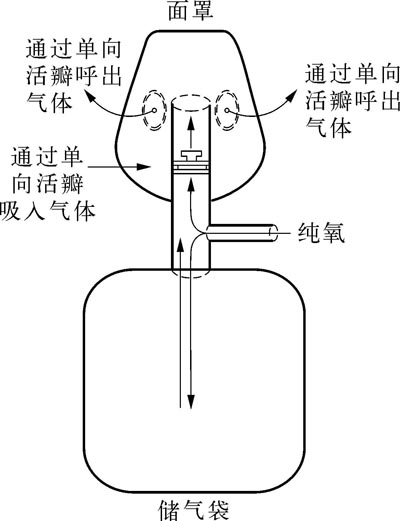
\includegraphics{./images/Image00073.jpg}
 \captionsetup{justification=centering}
 \caption{无重复呼吸面罩}
 \label{fig9-3}
  \end{figure} 

\subsubsection{应用Venturi面罩实施氧疗有何特点?}

可调式通气面罩即Venturi面罩(图\ref{fig9-4}),属于高流量氧疗系统,其吸入氧浓度可较好地控制。Venturi面罩可提供的吸入氧浓度为24%、26%、28%、30%、35%、40%。虽然Venturi面罩可提供40%以上的吸入氧浓度,但其精确度明显下降,与实测值可相差10%。低浓度时仅相差1%~2%。

\begin{figure}[!htbp]
 \centering
 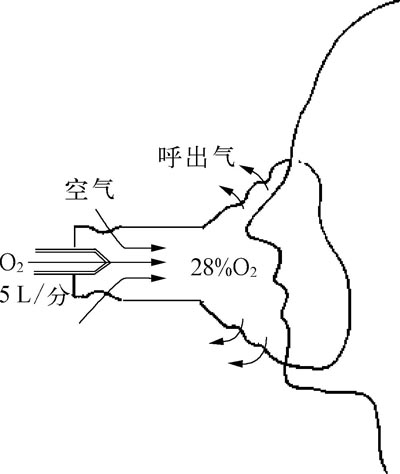
\includegraphics{./images/Image00074.jpg}
 \captionsetup{justification=centering}
 \caption{Venturi面罩}
 \label{fig9-4}
  \end{figure} 

可调式Venturi面罩具有如下优点:①可提供较恒定的吸入氧浓度;②由于喷射入面罩的气体流速超过患者吸气时的最高流速和潮气量,所以,患者呼吸模式变化不会影响吸入氧浓度;③可湿化氧气;④高流速气体可促使面罩中呼出气的二氧化碳排出,基本无二氧化碳重复吸入。Venturi面罩可适用于低氧血症伴高碳酸血症的患者。

\subsubsection{如何评价氧疗的效果?}

由于氧疗的目的是纠正组织缺氧,减少心肌和呼吸肌做功,因此,对氧疗效果的评价应包括对心肺系统的评估。

心血管系统评估主要应观察血压、脉搏和灌注状态。对于接受氧疗的患者,将其血压、脉搏与基础状态比较。如缺乏基础状态的资料,则应动态观察和评价。另外,心律失常可能是缺氧的后果,氧疗时也应注意。通过观察患者的皮肤颜色、湿度、温度和毛细血管再充盈时间,对灌注状态进行评估。每小时尿量及意识状态亦是反映危重患者组织灌注状态的重要指标。

呼吸系统的评估主要包括对潮气量、呼吸频率和呼吸功的观察和监测。临床观察判断潮气量往往不准确,如有可能应监测潮气量。观察呼吸频率,并注意呼吸节律是否规则。呼吸功为呼吸肌所做的功,降低呼吸功是氧疗的主要目的之一。当呼吸功增加时,患者往往有呼吸困难,并可表现为动用辅助呼吸肌。由于呼吸困难是呼吸功增加的重要主观指标,对于主诉有呼吸困难的患者,临床医师应特别重视。

动脉血气监测是评价氧疗效果的实验室指标。氧疗期间,应根据病情变化,反复监测动脉血气。根据动脉血氧分压水平,判断氧疗效果,并据此调整氧疗措施。另外,还应根据动脉血二氧化碳分压和pH值水平,判断患者的通气状态和酸碱平衡状态。

总之,鉴于氧疗的目的不仅仅包括纠正低氧血症,还包括降低呼吸功和心肌做功,故评价氧疗效果时应同时注意氧合和心肺功能状况。

\subsubsection{氧疗的吸入氧浓度为什么不宜超过50%?}

氧疗时,一般要求吸入氧浓度不宜超过50%,这主要与以下两个因素有关:

(1)吸入氧浓度高于50%可引起去氮性肺不张,导致解剖学分流增加。氧疗时,吸入氧浓度从21%逐步增加到50%,肺内总分流率(生理学分流和解剖学分流)明显降低,这与生理学分流被纠正有关,但进一步提高吸入氧浓度,总分流率反而明显增加。生理学分流随吸入氧浓度升高应进一步降低,总分流率增高必然与解剖学分流增加有关。去氮性肺不张是导致解剖学分流增加的主要原因。

正常情况下,氮气是维持肺泡膨胀的重要气体。存在生理学分流的肺泡,通气量不足,容积较小。当吸入氧浓度提高,特别是吸纯氧时,将发生以下两种效应:①通气不足的肺泡存在低氧性肺血管痉挛,当肺泡氧分压升高,其周围痉挛的毛细血管明显扩张,血流增加;②肺泡内氮气被洗出,氮气压力明显降低,肺泡内主要含有氧气。结果由于氧气迅速被吸收,这类肺泡便发生萎陷、形成肺不张、导致解剖学分流增加。吸入纯氧后15分钟就可发生去氮性肺不张,值得重视。总的来看,吸纯氧时的肺内分流率明显升高,而吸入氧浓度40%~60%时,肺内分流率最低(图\ref{fig9-5})。因此,一般情况下,实施氧疗时吸入氧浓度不宜超过60%。

\begin{figure}[!htbp]
 \centering
 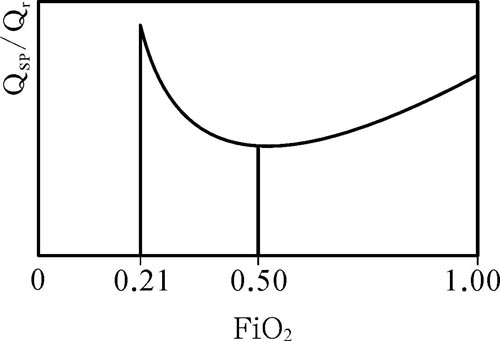
\includegraphics{./images/Image00075.jpg}
 \captionsetup{justification=centering}
 \caption{肺内总分流率与吸入氧浓度之间的关系}
 \label{fig9-5}
  \end{figure} 

(2)吸入氧浓度高于50%易导致氧中毒性肺损伤 氧中毒主要与吸入气中的氧分压有关。氧中毒的机理尚不甚明了,目前认为氧对细胞的毒性与其自由基毒性中间产物的作用有关,这些中间产物包括超氧自由基、过氧化氢、羟基自由基及单线态氧等活性氧。在1个大气压条件下,吸入空气可产生占氧耗量1%~5%的活性氧,其生成量随吸入氧浓度的升高而增加。在高浓度氧或高压氧疗时,产生活性氧的量超过了机体的处理能力,从而对机体细胞造成损害。氧中毒对肺的损害可表现为气管支气管炎、急性呼吸窘迫综合征、支气管-肺发育不良(见于新生儿)等。因此,从氧中毒的角度,对吸入氧浓度也应做出相应的限制。目前对氧浓度的安全界限尚无一致意见,但一般认为,在1个大气压条件下,吸入氧浓度低于60%的氧疗是无害的,长时间吸入氧浓度高于60%可能产生氧中毒,如吸纯氧,不应超过24小时。

\subsubsection{引起低氧血症的主要原因有什么?}

低氧血症是指在吸空气的条件下,动脉血氧分压低于80mmHg(1mmHg=0.133kPa)。可分为轻、中和重度低氧血症。动脉血氧分压60~80mmHg为轻度低氧血症,40~60mmHg为中度,低于40mmHg为重度。一般认为,动脉血氧分压36mmHg是人体生存的生理极限。低氧血症可引起广泛的组织细胞损伤,后果严重,是较常见的临床问题。引起低氧血症的原因主要包括以下两个方面。

(1)肺部疾病是导致低氧血症最常见的原因 可引起低氧血症的肺部疾病很多,主要包括以下几类------①肺泡通气量明显降低:严重的肺泡(低通气)可引起低氧血症,主要见于慢性阻塞性肺疾病、支气管扩张症等;②气体弥散功能障碍:主要见于肺纤维化、尘肺等;③通气/血流比例失调:为导致低氧血症最主要的原因,通气/血流比例<0.8者,依程度不同包括解剖学分流和生理学分流,见于肺不张、ARDS、肺实变等;通气/血流比例>0.8者为死腔样效应,主要见于肺栓塞等疾病。

(2)吸入气氧分压降低也是导致低氧血症的原因之一 这类情况主要见于高原居住或工作、高空飞行、潜水工作等。

\subsubsection{什么是顽固性低氧血症?其发生的主要原因是什么?}

顽固性低氧血症是指氧疗难以纠正的低氧血症,其诊断标准需符合以下指标之一:①吸入氧浓度高于35%的条件下,动脉血氧分压低于55mmHg;②吸入氧浓度提高20%(氧负荷试验),动脉血氧分压的升高不超过10mmHg。

引起顽固性低氧血症的主要原因包括:①解剖学分流明显增加。分流是导致低氧血症的主要原因之一,但生理学分流引起的低氧血症多能通过提高吸入氧浓度得到纠正,而解剖学分流引起的低氧血症,由于其通气/血流比例为0,氧疗难以奏效。解剖学分流增加主要见于心脏的右向左分流(例如先天性心脏病等)、肺动静脉瘘、肺不张、肺实变、ARDS等。正常情况下,解剖学分流不超过5%。病理条件下,解剖学分流高于30%时,将导致顽固性低氧血症。②严重的弥散障碍。严重的肺纤维化将导致肺泡-毛细血管膜增厚,气体弥散障碍,亦可导致严重的低氧血症。

\subsubsection{组织缺氧主要与哪些因素有关?氧疗是否一定能够纠正组织缺氧?}

组织缺氧不仅与呼吸性因素有关,还与血液、循环因素及细胞利用氧的能力有关。

氧输送减少是导致组织缺氧的主要原因。氧输送由动脉血氧含量和心脏指数决定,氧输送指数=动脉血氧含量×心脏指数。而动脉血氧含量由动脉血氧分压或动脉血氧饱和度和血红蛋白含量决定,动脉血氧含量=1.34×血红蛋白浓度×动脉血氧饱和度+0.0031×动脉血氧分压。从上述公式可以看出,以下三个因素均可导致氧输送降低,引起组织缺氧。

(1)呼吸性疾病引起低氧血症,即引起动脉血氧分压及血氧饱和度降低,使动脉血氧含量降低,导致氧输送降低。

(2)血红蛋白的质、量异常也是引起组织缺氧的重要原因。各种疾病引起的贫血,导致血红蛋白含量降低,使动脉血氧含量明显下降;另一方面,先天性血红蛋白异常、一氧化碳中毒、亚硝酸盐中毒时,血红蛋白含量可以正常,但因血红蛋白失去了结合氧的能力,也可导致动脉血氧含量降低。

(3)心脏是将富含氧气的动脉血送往组织的动力泵,心脏指数降低也是导致组织缺氧的重要原因。在动脉血氧分压和血红蛋白功能正常的情况下,心脏指数降低可引起氧输送降低,引起组织缺氧。这类情况主要见于左心衰及心包填塞引起的心源性休克、低血容量性休克等疾病。

需要指出,氧输送减少还包括氧输送的相对减少,即由于氧需或氧耗增加,导致氧输送尽管处于“正常水平”,但氧输送与氧耗失衡,仍然可引起组织缺氧。这类情况主要见于严重感染、高热、剧烈运动、甲状腺机能亢进等。

组织氧利用障碍也是造成组织缺氧的原因之一。组织细胞损害、酶系统功能障碍时,尽管氧输送正常,仍可引起组织缺氧。主要见于氰化物中毒、硫化氢中毒、休克引起组织细胞功能障碍等。

另外,血流分布及弥散等因素也与组织缺氧有关。感染性休克时,尽管心脏指数明显增加,但不同器官、组织的血流分布是不同的,某些组织可能血流减少而导致组织缺氧。氧从毛细血管弥散到细胞,取决于氧分压和弥散距离。组织水肿使弥散距离增大,可能加重组织缺氧。

综上所述,组织缺氧与动脉血氧分压、血红蛋白质量、心脏指数、组织氧利用能力等因素有关,其中只有动脉血氧分压降低或低氧血症引起的组织缺氧,可通过氧疗得以纠正,其他原因引起的组织缺氧氧疗难以奏效。因此,对于组织缺氧,应针对其原因,有的放矢地进行积极处理。

\subsection{人工气道的建立与管理}

\subsubsection{何谓人工气道,建立人工气道的指征是什么?}

人工气道是将导管直接插入气管或经上呼吸道插入气管所建立的气体通道。虽然人工气道的建立使患者失去了上呼吸道的加温、加湿、滤过功能,并削弱了自主清除呼吸道内异物的能力、不便于发音、降低患者的生活质量、增加院内感染的几率,但作为一种抢救的手段,人工气道的建立有利于痰液的引流、增进通气的有效性,导管气囊的存在可以使口咽部的分泌物、呕吐物不易进入肺部,并且能减少漏气,保证正压通气的有效实施。人工气道的应用指征应综合考虑循环、呼吸及中枢神经系统等方面的因素。一般而言,建立人工气道的指征如下。

(1)上呼吸道梗阻 口鼻腔及喉部软组织损伤、异物或分泌物潴留均可以引起上呼吸道梗阻,威胁患者生命。及时建立人工气道能够保证上呼吸道通畅。

(2)气道保护性机制受损 正常情况下,咽、喉、声带、气道及隆突通过生理反射(主要为迷走神经发射)对呼吸道发挥保护作用,依次存在咽反射(恶心和吞咽反射)、喉反射(声门关闭及会厌覆盖声门)、气管反射(异物或分泌物刺激气道引起咳嗽)及隆突反射(隆突受刺激而引发的强烈咳嗽)。患者意识改变(特别是昏迷)以及麻醉时,正常的生理反射受到抑制,导致气道保护性机制受损,易发生误吸及分泌物潴留,可能导致严重的肺部感染。因此,对于气道保护性机制受损的患者,有必要建立人工气道,以防止误吸和分泌物潴留。

(3)气道分泌物潴留 正常情况下,气道分泌物通过黏膜纤毛运动到达大气道,大气道受刺激后发生咳嗽反射,将分泌物咯出。正常的咳嗽反射受损时,会使分泌物在大气道潴留,易导致肺部感染和呼吸道梗阻。虽然可以经鼻腔或口腔将吸痰管插入咽部及气道,但往往效果很差,而且刺激性较大,患者不易配合,严重时还可以引起鼻咽部出血及诱发严重的心律失常。因此,及时建立人工气道,对清除气道分泌物是必要的。

(4)实施机械通气 需要接受机械通气的患者,首先应建立人工气道,提供与呼吸机连接的通道。当然,短时间实施正压通气,有时也可采取面罩与呼吸机相连,实施无创通气。但在需要长期机械通气或存在无创通气禁忌证时则必须建立人工气道,如呼吸心跳骤停、合并其他重要器官功能衰竭(严重脑病、严重上消化道出血、血流动力学不稳定或严重心律失常)、面部手术或创伤畸形、气道保护性机制丧失排痰障碍、严重低氧血症或酸中毒、近期上腹部手术等。

对指征的把握须进一步说明的是:①紧急建立人工气道无绝对禁忌证,关键在于选择最合适的方法,除非患者或法定监护人明确表示拒绝;②存在自主呼吸不是开放气道的禁忌证;③循环不稳定、严重酸中毒的患者,即使氧合尚可,从休克的复苏、纠正组织缺氧来说,也有指征早期开放气道正压通气;④建立人工气道和机械通气的指征不同,建立人工气道的患者不一定需要进行机械通气,但是进行有创机械通气必须先建立人工气道。

\subsubsection{紧急人工气道建立的适应证是什么?}

下列情况下需要紧急建立人工气道:①短时间内气道完整性受到破坏或气道梗阻;②呼吸衰竭需要呼吸机辅助呼吸;③紧急保护气道以防止可预见的影响气道通畅性的因素。

临床上需要建立紧急人工气道的常见危重病症包括深昏迷、呼吸衰竭或呼吸停止、心跳骤停、严重气道痉挛、气道异物梗阻、镇静剂或麻醉剂作用、颅脑及颈部外伤、误吸或有误吸危险(如上消化道大出血)、意外拔管、难以控制的上呼吸道出血、急性上呼吸道梗阻等。

\subsubsection{常见的人工气道有哪些类型?}

人工气道包括上人工气道和下人工气道。上人工气道包括口咽通气道和鼻咽通气道,有助于保持上呼吸道的通畅。口咽通气道适用于舌后坠而导致上呼吸道梗阻、癫痫大发作或阵发性抽搐,以及经口气道插管时,可在气管插管旁插入口咽气道,防止患者咬闭气管插管而发生部分梗阻或窒息。鼻咽通气道仅适用于因舌后坠导致的上呼吸道阻塞,但应注意凝血功能障碍者可能发生鼻咽出血。

最常用的人工气道是指下人工气道,主要包括气管插管和气管切开管。导管的材料、结构及应用的适应证均有所不同。

(1)气管插管导管

结构:气管导管为一略弯的管子,长度为28~32cm,内径为7.0mm、7.5mm、8.0mm等,内径越小,阻力越大,而且分泌物易阻塞管道。内径越大,阻力越小,但插管时较难通过鼻腔和声门,创伤性较大。导管远端开口呈45°斜面,带有单向活瓣的气囊,气囊充气后,阻塞导管与气管壁之间的间隙,可接呼吸机实施机械通气。

材料:气管导管有橡胶管、塑料管及硅胶管等几种。橡胶管质地硬,可塑性差,插管时易损伤鼻、声带及气管黏膜,更重要的是其组织相容性差,易导致黏膜充血、水肿、糜烂,甚至溃疡。聚氯乙烯塑料导管组织相容性好,受热后可软化,对上呼吸道的创伤性较小。硅胶导管的组织相容性更好,质地较软,但价格较贵。以往橡胶导管较常使用,目前很少使用,基本被塑料或硅胶导管替代。

气管导管气囊:气管导管气囊可分为高压低容和低压高容两种。气囊是否对气管黏膜有损伤作用,主要取决于气囊内压力及气管黏膜灌注压。高压低容气囊易导致黏膜缺血、糜烂、坏死、溃疡,已较少使用。低压高容气囊充气后,气囊内压较低,与气管黏膜接触面积大,对黏膜损伤较小,低压高容气囊是目前常用的气管导管气囊。

插管途径:有经口和经鼻气管插管两种。经口气管插管导管较粗,便于吸痰,急救时常常采用,但对于清醒患者常难以耐受,导管刺激口腔黏膜,分泌物较多,口腔护理困难,导管易移位而脱出,保留时间一般较短。经鼻气管插管比经口插管易于耐受、便于固定和口腔护理,导管保留时间较长,但经鼻插管对鼻腔创伤较大,易出血,采用的导管内径多偏小,而且导管弯度较大,使吸痰管插入困难,导管也易堵塞。

(2)气管切开管

结构:传统的气管切开管由内外套管组成,外套管带有单向活瓣的指示气囊。气管切开管通过固定带固定于颈部,内套管可与呼吸机相连接,而且便于拆卸,清洗管内分泌物和消毒,以保持呼吸道通畅。

材料:国产气管切开管多由银制的内外套管组成,使用逐渐减少。进口的塑料或硅胶套管更为常用,此类气管切开管无内套管。

气囊:气囊亦为低压高容气囊,对气管黏膜的损伤性较小。

\subsubsection{人工气道对患者有什么不良影响?}

人工气道是重要的抢救和治疗措施,但对患者也有不良影响。影响的程度与人工气道类型、使用时间、护理质量等有关。

(1)呼吸道的正常防御机制被破坏 正常情况下,机体通过上呼吸道的防御机制(湿化、滤菌、咳嗽、纤毛运动及杀菌等)防止细菌进入下呼吸道,使下呼吸道保持无菌状态。人工气道的建立,跨过了上呼吸道,使下呼吸道直接与外界相通,结果使气管支气管树易受细菌感染,导致肺部感染。

(2)抑制正常咳嗽反射 气管插管经过声门,使声带不能有效关闭,而气管切开管的气体通道又不经过声门,结果使机体咳嗽反射受到影响,患者不能有效咳嗽,其后果是分泌物在大气道潴留,误吸的分泌物也不能有效排除,极易发生肺部感染和呼吸道梗阻。

(3)影响患者的语言交流 气道插管或气管切开管的患者均不能发声,影响语言交流,常使患者感到孤独和恐惧,在重症医学科的特殊环境下尤为如此。可采用写字板等方式让患者进行有效交流。

(4)患者的自尊受到影响 对于神志清醒的患者,人工气道的建立常常使患者的自尊心受到伤害。经过人工气道呼吸,大量分泌物从人工气道直接排出、不能说话等,均使患者感到难堪。此时帮助患者建立自信是很必要的。

\subsubsection{经口气管插管的适应证和禁忌证有哪些?}

经口气管插管操作较容易,插管的管径相对较大,便于气道内分泌物的清除,但影响会厌功能,患者耐受性也较差。

经口气管插管适应证包括:①严重低氧血症或高碳酸血症,或其他原因需较长时间机械通气,又不考虑气管切开;②不能自主清除上呼吸道分泌物、胃内反流物或出血,有误吸危险;③下呼吸道分泌物过多或出血,且自主清除能力较差;④存在上呼吸道损伤、狭窄、阻塞、气管食管瘘等,严重影响正常呼吸;⑤患者突然出现呼吸停止,需紧急建立人工气道进行机械通气。经口气管插管的关键在于暴露声门,在声门无法暴露的情况下,容易失败或出现并发症。

禁忌证或相对禁忌证包括:①张口困难或口腔空间小,无法经口插管;②颈部无法后仰(如疑有颈椎骨折)。

\subsubsection{经鼻气管插管的适应证和禁忌证有哪些?}

经鼻气管插管较易固定,舒适性优于经口气管插管,患者较易耐受,但管径较小,导致呼吸功增加,不利于气道及鼻窦分泌物的引流。

经鼻气管插管适应证除紧急抢救外,均同经口气管插管。

经鼻气管插管禁忌证或相对禁忌证包括:①紧急抢救,特别是院前急救;②严重鼻或颌面骨折;③凝血功能障碍;④鼻或鼻咽部梗阻,如鼻中隔偏曲、息肉、囊肿、脓肿、水肿、异物、血肿等;⑤颅底骨折。

与经鼻气管插管比较,经口气管插管减少了医院获得性鼻窦炎的发生,而医院获得性鼻窦炎与呼吸机相关性肺炎的发病有着密切关系。因此,对短期内能脱离呼吸机的患者,应优先选择经口气管插管。但是,在经鼻气管插管技术操作熟练,或者患者不适于经口气管插管时,仍可以考虑先行经鼻气管插管。

\subsubsection{何谓逆行气管插管术?如何实施?}

逆行气管插管术是指先行环甲膜穿刺,送入导丝,将导丝经喉至口咽部,由口腔或鼻腔引出,再将气管导管沿导丝插入气管。

逆行气管插管术的适应证为:因上呼吸道解剖因素或病理条件下无法看到声带甚至会厌,无法完成经口或鼻气管插管。

禁忌证包括:①甲状腺肿大,如甲亢或甲状腺癌等;②无法张口;③穿刺点肿瘤或感染;④严重凝血功能障碍;⑤不合作者。

\subsubsection{经口气管插管的操作要点有哪些?}

经口插入气管插管是建立人工气道最常用的手段,也是心肺复苏时紧急建立有效气道的重要方法,因此,快速、准确的插入气管插管对于抢救患者显得十分必要。经口插入气管插管在操作上应注意以下要点。

(1)准备适当的喉镜 直接喉镜根据镜片的形状分为直喉镜和弯喉镜,使用方法上两者有所不同:直喉镜是插入会厌下向上挑,即可暴露声门;弯喉镜是插入会厌和舌根之间,向前上方挑,会厌间接被牵拉起来,从而暴露声门。耳鼻喉科医师为进行活检,需暴露充分,多采用直喉镜;而麻醉医师主要目的是插入气管插管,因此多采用弯喉镜。作为重症医学科医师,需适应各种急救环境,两种喉镜的使用方法均应掌握。

(2)准备不同型号的气管导管 准备不用型号的气管导管以备用,检查导管气囊是否漏气。可将气囊浸入生理盐水中,注入气体后检查是否漏气,然后将气体完全抽出。气管导管远端1/3的表面涂上石蜡油,将有助于插入声门,减少创伤。如使用导丝,则把导丝插入导管中,利用导丝将导管塑形。

(3)头颈部取适当位置是插管成功的主要保证 患者取仰卧位,肩背部垫高约10cm,头后仰,颈部处于过伸位,使口腔、声门和气管处于一条直线上,以利于插入气管插管。即使在紧急情况下,利用片刻时间,调整患者的体位也是十分必要的。

(4)预充氧、人工通气及生命体征监测 在准备插管的同时,应利用面罩和手动呼吸机或麻醉机,给患者吸入纯氧,同时给予人工通气,避免缺氧和二氧化碳潴留。当经皮血氧饱和度在90%以上(最好在95%以上)时,才能开始插管。如插管不顺利,或经皮血氧饱和度低于90%,特别是低于85%时,应立即停止操作,重新通过面罩给氧,并进行人工通气,直到血氧饱和度恢复后,再重新开始。插管前、插管过程中及插管后均应该密切监测患者的心电图和经皮血氧饱和度。

(5)插入喉镜,观察和清洁上呼吸道 操作者站在患者头端,用左手握喉镜,从患者口腔右侧插入,将舌头推向左侧。喉镜应处于口腔正中,观察口咽部。如有分泌物,则需充分抽吸,以免影响插管的视野。

(6)观察声门的解剖标志物 会厌和杓状软骨是声门的解剖标志物,会厌位于声门上方(前方),杓状软骨位于声门的下方(后方),两者之间即为声门。将喉镜插入会厌与舌根之间或插入会厌下方,向前上方挑,就可将会厌挑起,一般首先看到杓状软骨,再用力上挑,则可看到声带。气管插管时并非一定要看到声带,只要看到杓状软骨,甚至看到杓状软骨下方(后方)的食管,即可判断声门的位置,进行插管。

(7)插入气管导管,调节导管深度 观察到声门或声门的解剖标志物后,右手持气管导管,将导管插入声门。调整导管深度,避免插入过深,进入主支气管,注意双侧呼吸音是否对称。一般情况下,男性患者插入深度为距离门齿24~26cm,而女性为20~22cm。立即给气囊充气,将气管导管接呼吸机或麻醉机,实施机械通气,并吸入纯氧。使用导丝者,在气管导管插入声门后,一边送导管,一边将导丝拔除。

(8)确认导管插入气管 主要通过以下几种手段:①用听诊器听胸部和腹部的呼吸音,胸部呼吸音较腹部强;②监测患者呼出气二氧化碳浓度,如插入气管,则可见呼气时,呈现二氧化碳的方波;③对于有自主呼吸的患者,可通过麻醉机气囊的收缩,确认导管插入气管。

(9)固定气管导管 将牙垫插入口腔,此时才可将喉镜取出,用蝶形胶布将气管导管和牙垫一起固定于面颊部及下颌部。

(10)拍摄X线胸片,进一步调整导管位置 气管导管远端与隆突的距离应当为2~4cm。根据X线胸片,调整导管深度。同时观察患者肺部情况及是否并发气胸。

\subsubsection{如何判断气管导管是否插入气管?}

为保证气管插管插入气道内未误入食管,一个重要的经验是目睹气管插管管尖确实从声带之间进入。有时操作者看到了声门入口,但插管接近至声门处时,便移开了视线,结果气管插管误入食管。插管误入食管如不及时发现可能导致非常严重的后果(急性胃扩张,甚至胃穿孔或破裂。同时低氧血症也难以纠正)。判断气管导管是否插入气管的方法如下:

(1)观察通气时胸廓起伏及胃部情况,如果通气后胸廓起伏不明显,腹部明显膨隆,伴气管内胃内容物反流,则肯定不在气道。

(2)通气时听诊胸部和腹部呼吸音,如果胸部的呼吸音强,上腹部不明显,则考虑气管导管位于气管内。

(3)挤压胸廓,对于存在自主呼吸的患者则通过气管导管口听呼吸音,气流明显则提示多数在气管。

(4)接呼吸机看呼出气的流速波形,如果流速波形良好,则提示在气管内。

(5)监测患者呼气末二氧化碳,如插入气管,可见呼气时呈现二氧化碳方波;反之,如在食管内,则呼气末二氧化碳分压可降至或接近零。

(6)紧急床旁纤维支气管镜检查,如可见隆突及支气管开口,则确定在气管内。

在判断的过程中一定要注意血氧饱和度和心电的监测。对于不确定的或通气后生命体征更加不平稳的,应及时拔出导管,简易呼吸囊面罩加压充分氧合后再插管。

在上述方法中,以呼气末二氧化碳监测最准确,而呼气波形监测相对比较简单,且准确率高。

\subsubsection{气管插管插入气管的深度多少是合适的?}

(1)解剖长度 了解总气管长度以及从门齿至声门或至隆突的长度,有助于掌握合适的气管插管插入深度。门齿至声门或隆突的距离和年龄有关,见表\ref{tab9-2}。\footnote{*从成人的解剖长度,下列常数可供参考------①门齿至隆突的距离:男28.5cm,女25.2cm。②门齿至声门的距离:男12~16cm,女10~14cm。③从喉上缘至环状软骨下缘的距离:4~6cm。}

\begin{table}[htbp]
\centering
\caption{气管插管长度与门齿至声门或隆突距离\textsuperscript{*}}
\label{tab9-2}
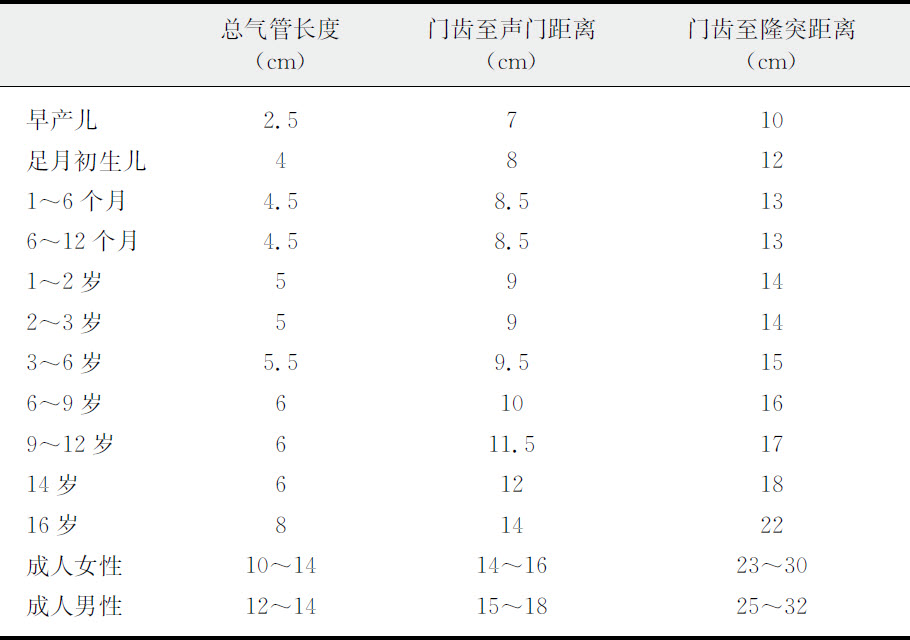
\includegraphics{./images/Image00076.jpg}
\end{table}

(2)插入合适深度 气管插管插入气管的深度,一般以气管插管尖到达气管中部,即位于声门下4~5cm(成人)较为合适。即使患者有仰头或低头,气管插管不致脱出声门;同时,气囊位于声门下,不会导致患者强烈的不适。

(3)插入深度的预估 为便于临床操作,气管插管插入合适深度有多种预估方法,这里介绍一种:①找出环状软骨(甲状软骨下方的软骨环);②再找出隆突的体表解剖位置,一般相当于平齐Louis角或第二肋软骨处;③确定环状软骨至隆突的中点;④将气管插管的管尖位置置于门齿水平,将插管弧度顺着患者颈部的侧面,直至环状软骨和隆突的中点,该长度就是气管插管插入气管的适当深度,若经鼻插管,则鼻孔入口处为测量的起点。

\subsubsection{在准备气管插管时,如何判断患者可能出现插管困难?}

气管插管为创伤性操作,如果插管前能够判断患者可能出现插管困难,则可以提前准备,以免不必要的反复插管,并避免发生严重并发症和医疗纠纷。

判断插管困难的主要手段和方法如下。

(1)观察咽部结构的可见程度 可用马兰帕蒂(Mallampatis)分级------患者用力张口和伸舌,窥视咽部结构:Ⅰ类,可见软腭、咽腭弓、悬雍垂;Ⅱ类,可见软腭、咽腭弓,悬雍垂被舌根遮盖;Ⅲ类,仅见软腭;Ⅳ类,可见硬腭,未见软腭。此试验仅能预测50%的插管困难,发生插管困难与软腭被舌根挡住有关。Ⅳ类和部分Ⅲ类者插管明显困难,除非头后仰受限,Ⅰ类和Ⅱ类者插管一般无严重困难。

(2)评价下颌骨颞骨关节活动度或张口度 成人最大张口时上下门齿间的距离正常为3.5~5.6cm,平均4.5cm。Ⅰ度张口困难者为2.5~3.0cm,技术娴熟的操作者仍可完成经口气管插管过程;Ⅱ度张口困难者为1.2~2.0cm,难以窥见咽喉部结构;Ⅲ度张口困难者<1.0cm,喉镜片无法置入口内。<1.5cm者无法用常规喉镜进行插管。张口受限可能原因为下颌关节病变或损伤、疤痕挛缩等。简易的评价方法是让患者张口,沿上下门齿方向插入手指,正常能够插入三横指。如不能插入三横指,则提示插管会遇到困难。

(3)评价寰椎枕骨关节的活动度 患者将口张开,上牙列水平与枕骨平面平行,然后将头部后仰,使下牙列水平与枕骨平行,头后仰的角度可反映寰椎枕骨关节的活动角度。寰枕关节正常时,可伸展35°以上,如活动角度降低1/3,则插管困难。据伸展度降低的程度分为4级:Ⅰ级伸展度无降低,活动角度>35°;Ⅱ级降低1/3,20°~25°;Ⅲ降低2/3,10°~12°;Ⅳ级伸展度明显降低,活动度<10°。寰枕关节伸展度降低可导致困难插管。

(4)颏甲间距 成人颈部完全伸展时,甲状软骨切迹至颏凸的距离,>6.5cm时不会发生插管困难;6.0~6.5cm时插管会有困难,但仍可能成功;<6.0cm时不能经喉镜插管。

(5)下颌骨水平支长度 指从下颌角至頦凸的长度,于9.0cm时发生插管困难的几率很小,<9.0cm时插管困难发生率很高,但此为国外资料,国人仅供参考。

(6)颈部后仰度 仰卧位下做最大限度仰颈,上门齿前端至枕骨粗隆连线与身体纵轴线相交的角度,正常>90°,<80°时颈部活动受限,插管可能困难。

(7)喉结过高 此时无法将口腔轴与喉腔轴调整为一个轴线水平,遇此情况插管可能困难。

(8)Cormack分级 用喉镜观察喉头结构:Ⅰ级,声门完全显露;Ⅱ级,声门部分显露,可见声门后联合;Ⅲ级,仅显露会厌或会厌顶端,不能窥见声门;Ⅳ级,声门及会厌均不能显露。这种分级与麻醉科医师的技术和经验有明显关系。Ⅰ级和Ⅱ级者一般不会发生插管困难;Ⅲ级和Ⅳ级者容易发生插管困难,导管误入食管的危险性达50%。

上述方法对判断气管插管是否困难有帮助,对其掌握可使操作者能够提早准备,但应用时仍应综合考虑。

\subsubsection{常规气管插管遇到困难时,有哪些对策?}

困难气管插管是指经过正规训练的医师使用常规喉镜正确地进行气管插管时,经3次尝试仍不能完成,这种情况发生率一般在1%~4%。

一旦判断可能发生困难插管,应采用以下插管方式:①普通喉镜清醒插管(表面麻醉、镇静、保持意识清醒、无呼吸抑制)。②纤维支气管镜引导插管,即气管导管套在纤维支气管镜外,直视下经声门进入气管,气管导管沿纤维支气管镜推入气管。③逆行引导清醒插管。④经口、鼻盲探插管。⑤面罩无创通气辅助下气管切开插管。⑥在插管困难时,可先置入喉罩,经喉罩通气管置入气管导管。当通气罩远端骑跨在声门裂上时,置入的气管导管应滑入气管。⑦指探引导法,即操作者站立在患者头部右侧,左手示指沿患者右口角后臼齿间伸入口腔抵达舌根,探触会厌上缘,并将会厌拨向舌侧。右手持气管导管插入口腔,在左手示指引导下,将管尖对准声门,患者吸气时将导管插入声门。

困难插管时须注意:①切忌惊慌,否则反而会延误处理问题的时机,只要保持患者有效通气和供氧,便不会有生命危险;②若没有其他插管方法,应通过封闭面罩简易呼吸囊加压给氧,辅助患者呼吸,患者自主呼吸恢复后,再考虑清醒插管;③插管操作应轻柔、准确、切忌使用暴力,同时避免长时间反复气管插管。

\subsubsection{心肺复苏时应采用什么方式建立人工气道?}

开放气道是心肺复苏的首要步骤。心肺复苏需要争分夺秒,要求人工气道的建立手段必须简洁、迅速,而且有效。目前常用的手段包括经口气管插管、面罩及食管阻塞器、环甲膜切开术。

经口气管插管是心肺复苏条件下建立人工气道的首选方法。作为紧急插管手段,经口气管插管简洁、方便,可迅速建立人工气道。

对于插管困难的患者,可采用面罩及食管阻塞器。食管阻塞器为一带气囊的、远端为盲端的管子。通过盲插,将气道阻塞器插入食管,气囊充气即可封闭食管,将面罩紧紧覆盖于患者口鼻部,则可实施正压通气。面罩及食管阻塞器的特点包括:①食管阻塞插管易插入食管;②用气囊封闭食管后,可防止胃内容物反流,也可防止正压气体进入胃肠道;③封闭性良好的面罩可保证正压通气的实施。

与其他人工气道相比,面罩及食管阻塞器存在一些问题:①需采用面罩,封闭性可能不佳,因此,实施正压通气不如传统的气管插管,但要优于简易呼吸囊面罩加压给氧。②拔除食管阻塞器时,往往有大量的胃内容物反流,易引起误吸。拔除食管阻塞器前应充分胃肠减压。③食管阻塞器可能引起食管穿孔、咽部及食管溃疡及声门上梗阻等严重的并发症;另外,食管阻塞器还可能插入气管,引起气道梗阻。

心肺复苏时,也可采用环甲膜切开术建立人工气道。手术时经正中切口切开环甲膜,可插入各种类型的通气管道,迅速建立人工气道。环甲膜切开术的主要优点有:①解剖标志明显,操作简单、迅速;②环甲膜位于声门之下,喉部大血管之上,因此,环甲膜切开不影响声门,而且出血少;③环甲膜切开位于气管上方,有必要时可择期进行气管切开。鉴于上述优点,环甲膜切开术被广泛推广应用,但多用于气管插管困难或无插管条件时,目前已有环甲膜切开包供临床使用。

\subsubsection{气管切开的适应证和禁忌证有哪些?}

气管切开术适应证为:①预期或需要较长时间机械通气治疗;②上呼吸道梗阻所致呼吸困难,如双侧声带麻痹、有颈部手术史、颈部放疗史;③反复误吸或下呼吸道分泌较多,患者气道清除能力差;④为减少通气死腔,利于机械通气支持;⑤因喉部疾病致狭窄或阻塞无法气管插管;⑥头颈部大手术或严重创伤需行预防性气管切开,以保证呼吸道通畅。气管切开术创伤较大,可发生切口出血或感染。

气管切开无绝对禁忌证,以下情况为相对禁忌证:①儿童;②颈部粗短肥胖,颈部肿块或解剖畸形;③颈部创伤(不稳定的颈椎骨折)或手术史;④甲状腺弥漫性肿大;⑤局部软组织感染或恶性肿瘤浸润;⑥难以纠正的严重凝血障碍;⑦需紧急建立人工气道。随着科技的进步和医学的发展,气管切开的指征在扩大,Kluge
S等
\protect\hyperlink{text00015.htmlux5cux23ch4-14}{\textsuperscript{{[}4{]}}}
研究显示,对于严重血小板减少患者经皮扩张气管切开也同样安全;Nun AB等
\protect\hyperlink{text00015.htmlux5cux23ch5-14}{\textsuperscript{{[}5{]}}}
\textsuperscript{,}
\protect\hyperlink{text00015.htmlux5cux23ch6-14}{\textsuperscript{{[}6{]}}}
研究显示,对于创伤患者同样可以行急诊气管切开。

\subsubsection{气管切开时机如何选择?}

对于需要较长时间机械通气的患者,气管切开是常选择的人工气道方式。与其他人工气道比较,由于其管腔较大、导管较短,因而气道阻力及通气死腔较小,有助于气道分泌物的清除,减少呼吸机相关性肺炎的发生率。但是气管切开的时机仍有争议。1989年美国胸科医师协会建议,预期机械通气时间在10天以内者应优先选择气管插管,而超过21天则应优先选择气管切开术,在10~21天之间者应每天对患者进行评估。当时这个建议尚缺乏临床研究的支持,是建立在专家经验之上的。之后,有研究比较了“早期”和“晚期”气管切开,探讨“最佳”气管切开时机,结果发现
\protect\hyperlink{text00015.htmlux5cux23ch12-14}{\textsuperscript{{[}12{]}}}
早期选择气管切开术,可以减少机械通气天数和重症医学科住院天数,同时可以减少呼吸机相关性肺炎的发生率。

对于“早期”的确切定义尚未统一,早至气管插管后48小时内,晚至气管插管后两周内,多数是在气管插管后7天或7天以内。Blot等
\protect\hyperlink{text00015.htmlux5cux23ch7-14}{\textsuperscript{{[}7{]}}}
对法国152个重症医学科病房机械通气的患者进行调查发现,气管切开的指征一般为机械通气20天或者拔管失败;早期气管切开的时间68%的<3周,平均为7天。Griffiths等
\protect\hyperlink{text00015.htmlux5cux23ch8-14}{\textsuperscript{{[}8{]}}}
的回顾性荟萃分析显示,早期气管切开(机械通气7天)可以降低机械通气时间和重症医学科住院时间,但不改变肺炎的发生率和病死率。

由此可见,对于需要长期机械通气或保留人工气道的患者可在7~10天行气管切开术,而对于脑血管病和颅脑外伤等患者,如预计短期内不能清醒的,气管切开时间可以更早,甚至在气管插管24小时以内。

\subsubsection{如何进行经皮扩张气管切开术?}

(1)术前准备 ①常规器械及药品准备:氧气,吸引器,面罩,喉镜,气管插管,气管切开包,纤支镜,抢救药品;②患者准备:适当镇痛镇静;③专用的经皮气管切开包:内含手术刀、带外套管的穿刺针、导引钢丝、扩张子、专用扩张钳、带气囊的气管切开套管等。

(2)体位及手术定位 ①体位:仰卧位,头后仰,肩部垫高,使下颏、喉结、胸骨上切迹三点一线,充分暴露颈部;②局部定位:选1~3气管软骨间(以甲状软骨为标志或胸骨上窝3~4cm),过高容易损伤环状软骨引起声门下的气管狭窄;过低容易损伤甲状腺峡部或无名动脉及其分支引起大出血。

(3)手术步骤 颈部消毒、局部麻醉后,横形切开皮肤1.5~2cm,在第1~2或2~3气管软骨间隙穿刺成功后置入导丝,以扩张子和扩张钳先后扩张皮肤、皮下和气管前壁(注意扩张钳角度),最后在导丝导引下置入气管套管,再次确认位置后,气囊充气并妥善固定(图\ref{fig9-6})。

\begin{figure}[!htbp]
 \centering
 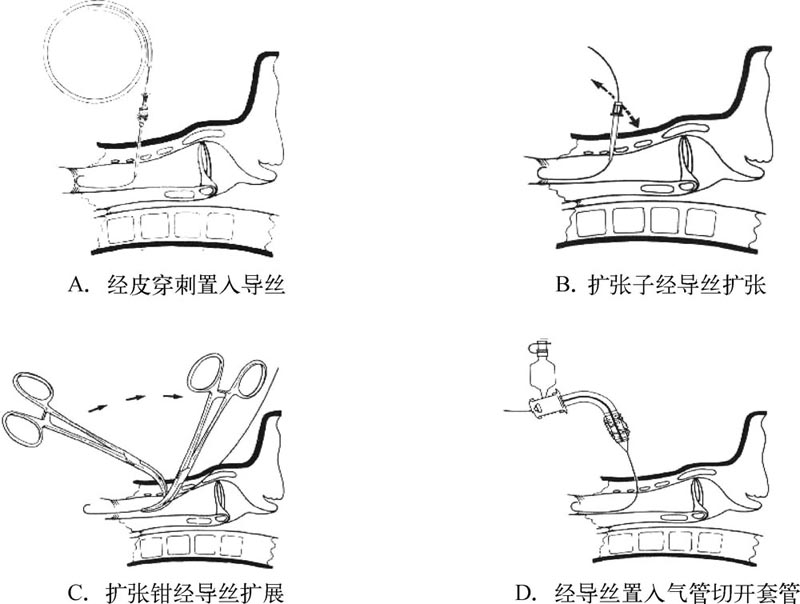
\includegraphics{./images/Image00077.jpg}
 \captionsetup{justification=centering}
 \caption{经皮扩张气管切开术的主要步骤}
 \label{fig9-6}
  \end{figure} 

\subsubsection{经皮扩张气管切开与经典的气管切开有何不同?}

(1)操作者不同 经典的气管切开由耳鼻喉科医师在直视下操作,通常在手术室进行,多需要麻醉医师协助;而经皮扩张气管切开术则一般由急诊科、重症医学科医师在床边操作。

(2)操作时间及并发症不同 荟萃分析显示,经皮气管切开手术操作时间短,一般为6~10分钟,术中及术后出血少,术后感染的并发症少,且易于床旁实施。

(3)费用不同 由于经皮气管切开可在床旁进行,无需单独的手术房间和专业的麻醉师,重症医学科住院时间相对短,费用相对低
\protect\hyperlink{text00015.htmlux5cux23ch3-14}{\textsuperscript{{[}3{]}}}
。

\subsubsection{应间隔多长时间更换气管切开管?}

气管切开管的更换时间尚无统一标准。一般认为,在气道充分湿化的条件下,应1~2周更换一次。也有专家认为,在气管切开窦口无明显感染的前提下,只要气管切开管无梗阻、功能正常,就可延长更换气管切开管的时间。当然,如果气管或气管切开窦口存在明显感染,应每周更换一次。如气管切开管出现部分梗阻或气囊破裂,则应立即更换。

\subsubsection{人工气道梗阻的常见原因有哪些?如何处理?}

人工气道梗阻是人工气道最为严重的临床急症,常常威胁患者生命。导致气道梗阻的常见原因包括:①导管扭曲,多与头颈部过度活动、经鼻插管、呼吸机管道牵拉等情况有关,调整头颈部位置后,气道梗阻常可改善;②气囊疝出而嵌顿导管远端开口,常见于头颈部位置改变或管道位置改变、气囊充气过多或气囊偏心、导管使用时间过长等,此时将气囊气体抽出,多可缓解气道梗阻;③痰栓或异物阻塞管道,见于痰栓或异物阻塞人工气道;④气道坍陷,多见于经鼻插管,特别是鼻中隔偏曲压迫管道;⑤管道远端开口嵌顿于隆突、气管侧壁或支气管,多见于导管插入过深或位置不当等,调整导管位置可能缓解气道梗阻。

一旦发生气道梗阻,应采取以下对策:①调整人工气道位置;②抽出气囊气体抽出;③试验性插入吸痰管。如气道梗阻仍不缓解,则应立即拔除气管插管或气管切开管,然后重新建立人工气道。若重新建立人工气道后,气道压力仍然很高,呼吸机不能进行有效的机械通气,则应当注意排除张力性气胸。

当然,积极采取措施预防气道梗阻可能更为重要,认真的护理、密切的观察、及时的更换管道及有效的人工气道护理,可对气道梗阻起到防患于未然的作用。

\subsubsection{建立人工气道的患者有哪些原因可导致气道出血?}

建立人工气道的患者出现气道出血,特别是大量鲜红色血液从气道涌出时,往往威胁患者生命,需要紧急处理。气道出血的常见原因包括:

(1)医源性因素是引起气道出血常见的原因,往往与吸痰管抽吸引起气道损伤有关。抽吸时负压作用于气管黏膜,引起黏膜损伤和出血,出血量往往不多。

(2)肺部感染也可引起气道出血,支气管肺炎和坏死性肺炎均可导致气道、肺内出血。

(3)急性心源性肺水肿可出现大量粉红色泡沫痰,当反复气道抽吸或存在出血倾向时,患者气道可涌出大量鲜红色血痰。

(4)少数患者可因肺栓塞而出现肺出血,可见于深静脉血栓脱落或深静脉导管相关的血栓脱落。

(5)肺动脉导管嵌顿时间过长亦可引起医源性肺梗死,而引起肺出血。另外,导管插入过深或飘入远端肺小动脉,气囊充气时可引起肺小动脉破裂而出血。

(6)气管导管和气管切开管气囊压迫腐蚀气道,可引起出血。最为严重的是,气囊压迫腐蚀引起无名动脉破裂出血,此种情况死亡率极高。

(7)出血性疾病或凝血功能障碍患者也常常出现气道出血。一旦出现气道出血,应针对原因,及时处理。

\subsubsection{气管切开可能出现哪些并发症?}

气管切开是建立人工气道的常用手段之一。由于气管切开后气流不经过上呼吸道,因此,与气管插管相比,气管切开具有许多优点:几乎没有上呼吸道的并发症;易于固定;易于呼吸道分泌物引流;附加阻力低,而且易于实施呼吸治疗措施;不影响经口进食,可做口腔护理;患者耐受性好。尽管具有上述优点,气管切开也可引起许多并发症,根据并发症出现的时间,可分为早期、后期并发症及拔管后并发症。以下着重讨论早期和后期并发症。

早期并发症指气管切开24小时内出现的并发症。常见的早期并发症如下。

(1)出血 是为最常见的早期并发症。出血凝血机制障碍的患者,术后出血发生率更高。出血部位可能来自切口、气管壁。气管切开部位过低,如损伤无名动脉,则可引起致命性的大出血。切口的动脉性出血需打开切口,手术止血。非动脉性出血可通过油纱条等压迫止血,一般在24小时内可改善。

(2)气胸 是胸腔顶部胸膜受损的表现,胸膜腔顶部胸膜位置较高者易出现,多见于儿童、肺气肿等慢性阻塞性肺疾病患者。上呼吸道梗阻患者,如梗阻未解除时实施气管切开,常常因存在过度肺充气、胸膜顶部位置高而易发生气胸。这类患者应首先插入气管插管,之后再行气管切开较为安全。

(3)空气栓塞 是较为少见的并发症,与气管切开时损伤胸膜静脉有关。由于胸膜静脉血管压力低于大气压,损伤时,空气可被吸入血管,导致空气栓塞。患者采用平卧位实施气管切开,有助于防止空气栓塞。

(4)皮下气肿和纵隔气肿 是气管切开后较常见的并发症。颈部皮下气肿与气体进入颈部筋膜下疏松结缔组织有关。由于颈部筋膜向纵隔延伸,气体也可进入纵隔,导致纵隔气肿。皮下气肿和纵隔气肿本身并不会危及生命,但有可能伴发张力性气胸,需密切观察。

后期并发症是气管切开24~48小时后出现的并发症,发生率可高达40%。主要包括:

(1)切口感染 这是很常见的并发症。感染切口的细菌可能是肺部感染的来源,故应加强局部护理。

(2)出血 气管切开后期也可发生出血,主要与感染组织腐蚀切口周围血管有关。当切口偏低或无名动脉位置较高时,感染组织腐蚀及管道摩擦易导致无名动脉破裂出血,为致死性的并发症。

(3)气道梗阻 是可能危及生命的严重并发症。气管切开导管被黏稠分泌物附着或形成结痂、气囊偏心疝入管道远端、气管切开管远端开口顶住气管壁等原因均可导致气道梗阻。一旦发生,需紧急处理。

(4)吞咽困难 这是较常见的并发症,与气囊压迫食管或管道对软组织牵拉影响吞咽反射有关。气囊放气后或拔除气管切开管后可缓解。

(5)气管食管瘘 临床偶见,主要与气囊压迫及低血压引起局部低灌注有关。

\subsubsection{如何预防和处理人工气道的意外拔管?}

意外拔管是指无拔管指征的患者,人工气道意外脱出。常见原因包括:患者烦躁或意识不清而意外拔管,固定不当,呼吸机管道牵拉及气管切开管过短等。意外拔管后患者可能出现以下情况:失去有效呼吸通道而发生窒息;完全依赖机械通气的患者则出现呼吸暂停;有自主呼吸的患者可能出现肺泡低通气等。无论出现哪种情况,均可能危及生命,因此,一旦发生意外拔管应紧急处理。

为避免意外拔管,须积极预防其发生,具体措施包括:①正确固定气管插管或气管切开管,每日检查,并及时更换固定胶布或固定带,气管切开管固定带应系方结,固定带应系紧,与颈部的间隙不宜超过两指;②检查气管插管深度,插管远端应距隆突2~3cm,过浅易脱出;③颈部较短的肥胖患者,如气管切开管较短,则头部活动时,易使导管脱出到皮下组织及脂肪组织中,引起呼吸道梗阻,此类患者宜选用较长的气管切开管;④对于烦躁或意识不清的患者,宜用约束带将其手臂固定,防止拔管;⑤呼吸机管道不宜固定过牢,应具有一定的活动范围,以防患者翻身或头部活动时导管被牵拉而脱出。

一旦发生意外拔管,应立即重建人工气道。气管切口3~5天内者,气管切开窦口尚未形成,气管切开管难以重新插入,可先行经口气管插管。对于气管插管困难者,可用简易呼吸囊面罩加压给氧,为进一步处理赢得时间。

\subsubsection{气管切开48小时内气管切开管意外脱出,应如何处理?}

在气管切开后48小时内,如气管切开管意外脱出,则不但换管困难,而且并发症较多。在气管切开48小时内,应注意以下问题:①由于气管切开窦道尚未形成,一旦拔出气管切开管,气管切开窦口将关闭,此后很难将气管切开管重新插入,由此可能引起呼吸道梗阻和严重缺氧,后果极为严重,应引起医护人员高度重视;②窦口肉芽组织尚未形成,重新插入气管切开管往往会引起出血;③气管切开管必须牢固固定,固定带应打死结,与颈部的间隙不应超过两指,另外,注意呼吸机管道不要过于固定,以免患者头颈部移动时,气管切开管被呼吸机管道牵拉而脱出;④患者床边应准备气管切开包、气管插管、简易呼吸囊等急救设备;⑤气管切开管一旦意外脱出或需紧急更换,应立即使用面罩和简易呼吸囊进行辅助通气,并吸入纯氧,保证患者的供氧和通气,如气管切开窦口漏气,可用纱布暂时封闭;⑥保证患者氧供的同时,立即呼叫耳鼻喉科医师,以便重新打开关闭的窦口,直视下插入气管切开管;⑦气管切开管重新插入前,必须认真检查气囊,以免插入后发现漏气而再次更换;⑧重新插入气管切开管后,必须认真固定管道。另外,意外拔管时,气囊上潴留的分泌物常常流入气管,引起误吸,可能导致或加重肺部感染,因此,必须彻底冲洗并抽吸气管;⑨整个操作期间,应注意监测患者心电图、经皮指脉氧饱和度和血压。

\subsubsection{如何调整气管插管或气管切开管气囊压力?}

由于气囊压力是决定气囊是否损伤气管黏膜的重要因素,调整气囊压力就显得特别重要。

正常成年人气管黏膜的动脉灌注压大约在30mmHg(42cm H\textsubscript{2}
O),毛细血管静脉端压力为18mmHg(24cm H\textsubscript{2}
O),淋巴管压力为5mmHg。由此可推测,气囊压力高于30mmHg时,气管黏膜血流将完全被阻断,可引起黏膜缺血;当气囊压力高于18mmHg,将引起气管黏膜静脉回流受阻而出现淤血;当气囊压力高于5mmHg时,将阻断淋巴回流,引起黏膜水肿。气囊充气过多,压力过高,会引起黏膜损伤;而压力过低则不能有效封闭气囊与气管间的间隙。因此,必须注意调整气囊压力,避免压力过高或过低。理想的气囊压力为有效封闭气囊与气管间隙的最小压力,常常称为“最小封闭压力(MOP)”。目前推荐气囊压力>20cm
H\textsubscript{2} O,一般维持在25~35cm H\textsubscript{2}
O,可以通过Portex气囊压力测定仪进行调整,一般每天监测2~3次气囊压力,避免气囊压力过高或过低。

\subsubsection{为什么气管插管或气管切开管气囊不需定期放气?}

以往认为,气管插管或气管切开管气囊应常规定期放气-充气,其主要目的是通过放气(多为3~5分钟)恢复气管黏膜血流,防止气囊压迫导致气管黏膜损伤。

目前认为,气囊定期放气-充气是不必要的,主要依据如下:

(1)气囊放气后,1小时内气囊压迫区的黏膜毛细血管血流也难以恢复。气囊放气5分钟不可能恢复局部血流。可见,短时间气囊放气不能达到恢复黏膜血流的目的。

(2)声门与气囊之间的间隙常常有大量分泌物潴留,定期气囊放气有可能增加了反复误吸的可能性。

(3)对于机械通气支持条件比较高的危重患者,特别是依赖于高水平呼气末正压(PEEP)的呼吸衰竭患者,气囊放气将导致肺泡通气不足,PEEP不能维持,并可能引起循环波动,因此,危重患者往往不能耐受气囊放气。

(4)常规的定期气囊放气-充气,往往使医师或护士忽视气囊容积或压力的调整,反而易出现充气过多或压力过高的情况。

虽然人工气道气囊不需常规放气-充气,但某些情况下,非常规性的放气或调整仍然是必要的。气囊放气及重新充气主要用于以下情况:

(1)气道峰值压力是影响气管最大内径的主要因素,当气道峰值压力明显升高或降低时,为避免气囊压力(或容积)过高或过低,应将气囊放气,重新充气,并测定气囊压力,保持在20~35cm
H\textsubscript{2} O。

(2)人工气道的建立破坏了呼吸道的正常解剖和功能,声门与气囊之间的间隙成为一死腔,常常有大量分泌物在此潴留,可能形成隐匿感染灶。因此,经常清除这些分泌物,保持声门下和气囊上区域的清洁是十分必要的。研究表明,有效的声门下吸引可降低呼吸机相关性肺炎的发生率
\protect\hyperlink{text00015.htmlux5cux23ch11-14}{\textsuperscript{{[}11{]}}}
。对于不带声门下吸引的普通导管,清除气囊上分泌物的方法之一就是在气囊放气的同时,通过呼吸机或手动简易呼吸囊,经人工气道给予较大的潮气量,在塌陷的气囊周围形成正压,将潴留的分泌物“冲”到口咽部,从而达到既清除气囊上分泌物,又防止了气囊放气后分泌物流入气管的目的。

\subsubsection{人工气道患者实施气道抽吸时,应如何选择适当的吸痰管?}

吸痰时,为避免黏膜创伤及继发感染,应选择适当的吸痰管。吸痰管应符合以下要求:①吸痰管材料应对黏膜的损伤小;②吸痰管摩擦力小,以利于通过人工气道;③足够的长度,使吸痰管远端应能达到人工气道远端或隆突,否则难以达到抽吸气道分泌物的目的;④远端光滑,而且应该为侧开口,以减少对黏膜损伤;⑤吸痰管近端应有足够大的侧孔,需要中断负压吸引时,只要开放侧孔即可,可避免负压持续吸引引起黏膜损伤或肺不张,也可避免反复关闭负压吸引器;⑥吸痰管直径(外径)不应超过人工气道内径的一半,如吸痰管直径过大,负压吸引时,吸痰管周围卷入的空气较少,易导致肺萎陷或肺不张;⑦吸痰管应无菌、单根包装,以避免交叉感染,而且操作方便,如有条件,应使用一次性吸痰管。

\subsubsection{呼吸道负压抽吸吸痰的操作要点是什么?}

为减少气管损伤、感染等并发症,经人工气道进行呼吸道负压引流(吸痰)时应注意以下操作要点:

(1)注意无菌操作,拿吸痰管时应戴无菌手套,使用无菌的吸痰管,应用无菌的冲洗盐水等。绝对禁止用抽吸口鼻腔的吸痰管再抽吸气道。

(2)吸痰前必须预充氧,使体内获得氧贮备。通过手动呼吸,吸入高浓度氧。接受机械通气的患者,可通过吸入纯氧3~5分钟达到预充氧的目的。充分的预充氧,可避免发生低氧血症。

(3)吸痰管插到气管插管远端前,不能带负压,以免过度抽吸肺内气体,引起肺萎陷。

(4)插入吸痰管过程中,如感到有阻力,则应将吸痰管后退1~2cm,以免引起支气管过度嵌顿和损伤。

(5)在吸痰管逐渐退出的过程中,打开负压吸痰,抽吸时应旋转吸痰管,并间断使用负压,可减少黏膜损伤,而且抽吸更为有效。

(6)吸痰管在气道内的时间不应超过10~15秒,而从吸痰过程开始到恢复通气和氧合的时间不应超过20秒。

(7)抽吸期间应密切注意心电监测,一旦出现心律失常或呼吸窘迫,应立即停止抽吸,并吸入纯氧。

(8)通气和氧合恢复后至少进行5次深呼吸,生命体征恢复到基础水平后,才可再次抽吸。

(9)经反复抽吸,应较彻底地清除分泌物。

(10)气道抽吸后,可使用同一吸痰管抽吸口、鼻、咽腔,但抽吸过口鼻咽腔后,绝不可再抽吸气管。

(11)气道分泌物的抽吸不应作为常规操作,当患者有气道分泌物潴留的表现时,才有指征抽吸。过多的抽吸会刺激、损伤气道黏膜。

\subsubsection{呼吸道负压抽吸吸痰应注意哪些并发症?如何处理?}

由于人工气道影响患者正常咳嗽反射,大气道内的分泌物必须通过抽吸清除。对于危重患者,吸痰时的抽吸技术不当,可能引起严重的并发症,甚至引起心脏骤停,因此,了解气管吸痰过程中的有关并发症,对于防止和及时处理并发症都是十分必要的。

(1)低氧血症 多数带有人工气道的患者需接受不同程度的氧疗,以维持动脉血氧分压。吸痰时,吸痰管插入气道,负压抽吸将肺内的富氧气体吸出,而从吸痰管周围卷入的气体是氧浓度较低的空气,容易导致低氧血症。对于危重患者,低氧血症的恶化往往会威胁患者生命。

吸痰导致的急性低氧血症往往表现为心率改变。多数患者表现为心动过速,重新吸入高浓度氧气后,心率逐渐降低。少数患者表现为心动过缓。在吸痰过程中,心率及心律的任何改变均应考虑与低氧血症有关。

吸痰前通过提高吸入氧浓度(预充氧),提高机体内氧贮备是防止低氧血症的重要措施。另外,应用封闭式吸痰管使吸痰时不中断氧疗(不脱开呼吸机或氧疗系统),也可一定程度上防止低氧血症。

(2)心律失常 吸痰过程中发生的严重心律失常,主要与低氧血症引起心肌缺氧或气管黏膜受刺激后导致迷走神经兴奋有关,这两个因素哪个更为重要目前尚不清楚。抽吸过程中出现的室性早搏等严重心律失常,可能与这两因素均有关,而明显的心动过缓主要由迷走神经兴奋引起。如操作适当,可减少心律失常发生的可能性。

(3)低血压 吸痰过程中常常发生血压降低,可能与迷走神经兴奋引起心动过缓有关,也可能与连续咳嗽有关。吸痰管刺激气管黏膜或隆突,引起气管或隆突反射,会使患者出现阵发性咳嗽样动作,并伴有心动过缓,导致静脉回流和心输出量均明显降低,结果出现低血压。

(4)肺萎陷或肺不张 负压抽吸时,如吸痰管周围没有足够的空气卷入,容易导致肺萎陷或肺不张。吸痰管直径过大(超过人工气道内径一半)或负压过大时易于发生。因此,选用适当直径的吸痰管,并采用合适的负压是有必要的。

\subsubsection{如何实现左主支气管的选择性抽吸吸痰?}

由于左主支气管从气管发出的角度较小,吸痰管不易进入。吸痰时,吸痰管是否能够进入左主支气管,主要取决于以下条件:①人工气道的类型。与气管插管相比,经气管切开管吸痰更易进入左主支气管。②头的位置。头转向右侧,吸痰管易进入左主支气管。③吸痰管的类型。弯头吸痰管较易进入左主支气管。需要抽吸左主支气管时,应根据上述情况,选择适当的吸痰管和体位。

\subsubsection{何谓气道湿化?正常上呼吸道的湿度如何?}

气道湿化是指应用湿化器及其他装置将溶液或水分分散成极细微粒,以增加吸入气中的湿度,使气道和肺部能吸入含足够水分的气体,湿化气道黏膜、稀释痰液、保持黏液纤毛正常运动和廓清功能。

气道湿化时经常用到“湿度”这一物理学概念。所谓湿度即空气中所含水分的多少或潮湿程度。单位容积的气体中所含水分的重量称之为绝对湿度,常用计量单位为mg/L或g/m\textsuperscript{3}
。在一定温度下,气体实际所含水分与该温度下每单位容积所能容纳的最大水分含量的比值称为相对湿度,可用湿度计进行测量。

正常呼吸过程中,上呼吸道将干燥、温度较低的空气,逐步转化为湿润温暖的气体后到达肺泡进行气体交换。一般空气的温度21℃,相对湿度为50%,吸入气体经过鼻腔、咽喉到达气管上段时,温度已达34℃,相对湿度为100%,绝对湿度36~40mg/L;到达气管隆突时,温度约37℃,相对湿度为100%,绝对湿度约43.9mg/L。可见,人体在吸入空气时,呼吸道必须对空气进行加温加湿,生理情况下这一过程由上呼吸道完成。正常成人经气道蒸发的水分约为250ml/天,当遇到发热、过度通气或吸入干燥空气后水分丢失更多。人工气道的建立,使患者在吸气过程中丧失了上呼吸道对吸入气体的加温加湿功能,为维持相应的状态必须进行充分的气道湿化。

\subsubsection{气道管理中为什么要重视气道湿化?}

人工气道的建立,使危重患者在吸气过程中丧失了上呼吸道对吸入气的加温和加湿功能,只能吸入干燥和温度较低的空气,结果吸入气的湿化和加温功能由气管支气管树黏膜来完成,因气体湿化不足,易引起气管黏膜干燥、分泌物黏稠而形成痰栓,导致多种严重后果,这主要包括:①黏膜纤毛运动受损;②黏液的移动受限;③气管支气管黏膜上皮发生炎症性改变甚至坏死;④黏稠分泌物潴留,进而形成痰痂,严重者可发生气管梗阻;⑤细菌易浸润气管黏膜,导致肺部感染;⑥黏稠分泌物阻塞小气道,易发生肺不张。由此可见,人工气道的管理中,必须强调给予充分的气道湿化,防止可能发生的不良后果。由于湿化的主要目的是替代上呼吸道的加湿和加温功能,因此,经湿化的气体相对湿度应当达到100%,温度应达到35~37℃。

当然,过度加温和湿化也可造成有害的影响,这包括:①湿化器温度过高,可以引起气道黏膜温度过高或烧伤,导致肺水肿和气道狭窄;②如果吸入的气体没有加热,但直接经呼吸道给予大量水分,会由于需要蒸发消耗热量而导致体温下降、体液负荷增加、黏膜纤毛的清除功能减退。

\subsubsection{气道湿化有哪些适应证和禁忌证?}

适应证为:①未建立人工气道而使用干燥的医疗气体者,如对于吸氧流量超过4L/分钟的;②建立人工气道者;③高热、脱水;④呼吸急促或过度通气;⑤痰液黏稠或咯痰困难;⑥气道高反应,部分原因是由于干冷气体诱发的气道痉挛;⑦低体温,尤其是低温冻伤在复温过程中的机械通气患者。

气道湿化无绝对禁忌证。气道分泌物过多且稠厚或血性分泌物时应慎用气道湿化,以免加重气道梗阻,甚至窒息。

\subsubsection{保持呼吸道湿化的常用方法有哪些?}

(1)保证充足的液体入量 机械通气时,液体入量应保持每日2500~3000ml。呼吸道湿化尽量以全身不脱水为前提,如果机体液体入量不足,即使呼吸道进行湿化,呼吸道的水分会进入到失水的组织中,呼吸道仍可能处于失水状态,所以,必须补充足够的液体入量。

(2)加温湿化器 加温湿化器以物理加热的办法为干燥气体提供恰当的温度和充分的湿度,能使湿化后的气体达到100%的湿度。湿化罐温度的控制应以气管插管或气管切开管处的气体温度达到37℃为准,因此,监测气管插管或气管切开处的气体温度是必要的。湿化加水时,应加无菌的蒸馏水或注射用水,注意整个操作过程保持无菌。管路内凝结的水,若意外地灌进患者的气道,可成为医院感染的来源,因此管内的冷凝水应收集于积水瓶中,并及时清除,也不能使冷凝水流回湿化器。

(3)湿热交换器 也称人工鼻。该装置放置在“Y”形管与气管导管之间,为被动湿化。工作原理为随温度的变化,携水能力有连续性变化。呼气时,随温度的下降,呼出的水分被截留在人工鼻中;吸气时,温度逐渐升高,人工鼻的水分补充到吸入气体中。优点包括:①保证黏液纤毛系统运动正常;②减少热量丧失;③保证管路干燥,减少细菌孳生,防止感染的发生;④操作简单,可以不需要每日更换,减少如加温湿化器因需加水而多次管路断开导致的交叉感染。但近期研究显示,湿热交换器并不能降低呼吸机相关性肺炎的发生率
\protect\hyperlink{text00015.htmlux5cux23ch10-14}{\textsuperscript{{[}10{]}}}
\textsuperscript{,}
\protect\hyperlink{text00015.htmlux5cux23ch11-14}{\textsuperscript{{[}11{]}}}
。在有下列情况的患者人工鼻不适用:分泌物黏稠或血性,患者中心体温<32℃,呼出潮气量<吸气潮气量的75%(如气管胸膜瘘等),呼出潮气量>10L/分钟,咯血,撤机困难等。

(4)雾化器 临床有喷射式雾化器和超声雾化器,通过雾化器将湿化液激发为微粒或雾粒,悬浮在吸入气流中一起进入气道而达到湿化气道的目的。雾化器产生雾粒的量和平均直径的大小,随雾化器种类而不同。

(5)气道冲洗 常用生理盐水,在吸痰前予2~5ml生理盐水在吸气末注入气道。操作前,先给予纯氧2~3分钟,以免造成低氧血症。注入冲洗液后,给予吸痰或配合胸部叩拍,使冲洗液和黏稠的痰液混合震动后再吸出。全天湿化液总量一般不超过250ml。

\subsubsection{机械通气时人工气道的主动湿化和被动湿化有何不同?}

机械通气时的气道湿化包括主动湿化和被动湿化。主动湿化主要指在呼吸机管路内应用加热湿化器进行呼吸气体的加温加湿(包括不含加热导线,含吸气管路加热导线,含吸气呼气双管路加热导线);被动湿化主要指应用人工鼻(热湿交换器型)吸收患者呼出气的热量和水分进行吸入气体的加温加湿。不论何种湿化,都要求进入气道内的气体温度达到37℃,相对湿度100%,以更好地维持气道黏膜完整,纤毛正常运动及气道分泌物的排出,降低呼吸道感染的发生。人工鼻(热湿交换器型)可较好进行加温加湿,与加热型湿化器相比不增加堵管发生率,并可保持远端呼吸机管路的清洁,但可能增加气道阻力、死腔容积及吸气做功,不推荐在慢性呼衰患者尤其是有撤机困难因素的患者应用。有研究认为,人工鼻(热湿交换器型)较加热型湿化器能减少院内获得性肺炎的发生,但近年来多个随机对照临床研究认为,人工鼻与加热型湿化器比较,在呼吸机相关性肺炎的发生率上无明显差异。

\subsubsection{气道湿化效果如何判断?}

湿化效果应根据患者的自觉症状和监测指标变化来判断,同时应把这些自觉症状和监测指标的变化与病情相结合,防止误判或延误患者的治疗。一般把湿化效果归为以下3种:

(1)湿化满意 ①痰液稀薄,能顺利吸出或咯出;②人工气道内无痰栓;③听诊气管内无干鸣音或大量痰鸣音;④呼吸通畅,患者安静。

(2)湿化过度 ①痰液过度稀薄,需不断吸引;②听诊气道内痰鸣音较多;③患者频繁咳嗽,烦躁不安,人机对抗;④可出现缺氧性紫绀、经皮指脉氧饱和度下降及心率、血压改变等。

(3)湿化不足 痰液黏稠,不易吸出或咯出;听诊气道内有干鸣音;人工气道内可形成痰痂;患者可出现突然的吸气性呼吸困难、烦躁、紫绀及脉搏氧饱和度下降等。

\subsubsection{气管插管或气管切开管的拔管指征是什么?}

总的说来,当建立人工气道的原发病得到控制时,就有拔除气管插管或气管切开管的指征。与建立人工气道的指征类似,拔管指征也从4个方面进行考虑。

(1)引起上呼吸道梗阻的因素已去除 当上呼吸道梗阻的病因缓解后,可考虑拔管,但拔管后应密切观察患者是否在此重新出现上呼吸道梗阻的症状。中枢神经系统受损是引起上呼吸道梗阻的常见原因,中枢神经功能改善将使上呼吸道梗阻改善。

(2)气道保护性反射恢复 气道保护性反射受影响的顺序,从重到轻依次为咽、喉、气道及隆突反射,因此,评价气道保护性反射是否恢复,可观察咽反射是否恢复。带管情况下,如果患者存在吞咽反射(咽反射的表现),则喉、气管及隆突反射应当是正常的,这是安全拔管的前提。

(3)具有呼吸道清洁能力 是否需要气道抽吸清除分泌物,在很大程度上是由患者咳嗽能力决定的。对患者咳嗽能力的评价,可通过观察患者咳嗽的强度、肺活量、最大吸气负压及意识水平来决定。如果患者在带管情况下具有一定咳嗽能力,肺活量接近正常,而且患者能够合作,则拔除人工气道后,患者大多具有气道清洁能力。

(4)已撤离呼吸机 如建立人工气道的主要目的是实施机械通气,又在撤离呼吸机后符合上述条件,则可考虑拔除人工气道。

在此需要说明的是,脱机与拔除人工气道是两回事,部分患者经过治疗后可以脱离呼吸机,但因气道自洁能力差,仍需要人工气道;而另外一部分患者,如慢性阻塞性肺疾病,即使不符合拔管条件,但在感染控制窗内仍可以考虑拔除气管插管,实施有创通气无创通气序贯脱机。

\subsubsection{如何正确地拔除气管插管?}

对于有拔除气管插管指征的患者,一旦决定拔管应遵循以下操作过程:

(1)拔管后患者的合作十分重要。拔管前应让患者了解拔管的必要性和安全性,消除患者心理负担,使其充分合作,另须准备好吸氧装置、口腔护理物品、纸巾、雾化装置,必要时备无创通气。

(2)彻底、充分地吸引气道分泌物之后,清除口咽及鼻咽部分泌物,如为带声门下引流的导管,应充分冲洗抽吸声门下引流管;如为普通导管,可通过在气囊放气的同时,通过呼吸机或简易呼吸囊,经人工气道给予较大的潮气量,以期在塌陷的气囊周围形成正压,将潴留的分泌物“冲”到口咽部,再给予吸出,避免误吸。

(3)适当提高吸入氧浓度,增加体内氧贮备。

(4)让患者深呼吸数次或通过简易呼吸囊给予较大潮气量,以鼓肺,复张塌陷肺泡,改善肺不张。

(5)将新的吸痰管置于气管插管远端开口以远1~2cm,边抽吸,边气囊放气,并快速拔除气管插管。

(6)采用合适的氧疗措施及口腔护理。

(7)立即评价患者气道是否通畅,有无气道梗阻的症状,有无喘鸣或呼吸困难,鼓励患者做深呼吸。

(8)病情完全稳定前,应给予特别护理。床边应备有急救设备。

另外,为防止声门及声门下水肿,在拔管前可给予肾上腺素雾化吸入或地塞米松雾化吸入或静脉注射。

\subsubsection{人工气道拔除后发生喉头水肿应如何处理?}

喉头水肿是气管插管拔管后最严重的并发症之一,严重者可危及生命,需要紧急处理。喉头水肿实际上是指声门区域发生水肿。儿童的发生率远高于成人。如能早期认识、早期处理,多数患者不需再插管。

引起喉头水肿的主要原因包括:①插管及留置期间对声门区域有损伤;②气管插管内径过大;③气管插管护理不当;④导管引起的过敏反应。

轻度喉头水肿无症状。当喉头水肿引起声门狭窄,声门截面积小于正常50%时,患者出现临床症状,主要表现为吸气期喘鸣、呼吸困难,并进行性加重。由于喉部位于胸腔外,自主呼吸时吸气期声门最为狭窄,所以,患者在吸气期出现喘鸣。一般在气管插管拔除后随即出现症状,水肿在数小时内达到极限,而后逐渐缓解。当然,拔管后无喉头水肿症状立即出现,并不意味着患者就不再会发生喉头水肿,故在拔管后24小时内均应警惕。

一旦出现喉头水肿症状,应积极治疗,以防进一步恶化。主要治疗措施包括:①吸入室温的雾化气体,以保证声门区域充分湿化,同时减轻对黏膜的刺激,减轻毛细血管水肿和充血;②局部应用血管收缩药物,如麻黄素、肾上腺素雾化吸入或直接喷入咽喉部;③静脉注射地塞米松等糖皮质激素类药物,以改善声门水肿,也可局部用药;④当上述措施不能奏效或气管梗阻很严重时,应立即重新建立人工气道。

\subsubsection{人工气道拔除后发生气管狭窄的主要原因有哪些?}

在人工气道(气管插管或气管切开管)建立后1周至2年期间,均有可能发生气管狭窄。气管狭窄是气管局部损伤愈合过程中,瘢痕组织收缩的结果。有的患者同时伴有气管软化,即气管软骨被破坏,表现为吸气时气管塌陷。气管狭窄的发生部位主要在气囊压迫部位。临床研究调查发现,使用不带气囊的气管切开管,气管狭窄的发生率低于2%,而使用带气囊的气管切开管时,气管狭窄的发生率可达5%。机械通气患者的调查发现,气管狭窄发生率为1%~65%。结果的差异性与研究方法、气管狭窄的诊断标准及研究人群不同等因素有关。一般认为,气管内截面积减少50%以上,气管狭窄患者才出现喘鸣、呼吸困难、活动能力下降等临床表现。

气管狭窄的发生部位似乎提示气囊是引起气管狭窄的主要原因,但临床观察及动物实验研究显示,气管狭窄不仅与气囊有关,还与其他许多因素相关。总的来说,是否发生气管狭窄主要与以下因素有关。

(1)气囊压力过高是导致气管狭窄最重要的因素之一 气囊压力过高可引起气管黏膜水肿、淤血及缺血,进而可能引起黏膜发生糜烂、溃疡。基于这一认识,须强调气囊压力的监测和调整。

(2)人工气道的维持时间也是引起气管狭窄的因素 人工气道维持的时间越长,气管狭窄的发生率越高、越严重.

(3)低血压低灌注是导致气管狭窄发生的重要因素 休克或一过性低血压可引起气管黏膜灌注降低,使气囊压迫部位的气管黏膜易发生缺血、坏死,因此,防止并及时纠正休克是防止气管狭窄的重要环节。

(4)局部感染也是导致气管狭窄的原因之一 建立人工气道的患者,气管内细菌定植是难以避免的,易继发感染。当然,良好的气道护理可防止急性气管感染发生。调查显示,感染虽然不是气管狭窄的主要原因,但增加气管狭窄的发生率。

(5)人工气道的活动、牵拉或负重等因素也增加气管狭窄的发生率 人工气道的活动、牵拉或负重可导致气管切开窦口周围压力增高及气囊移位,并刺激气管黏膜,结果气管黏膜易发生缺血坏死。可见有必要采取措施,适当固定人工气道,可采用支撑架托住气管插管或气管切开管,同时支撑架需要有一定的活动度,患者头颈部移动时人工气道不致被牵拉。

(6)人工气道对人体组织的毒性作用也可能与气管狭窄有关 如人工气道的组织相容性不佳,则可能造成周围气管组织发生炎症反应。

针对上述导致气管狭窄的原因,应采取相应的对策,以防止气管狭窄的发生。

\subsection{胸部物理治疗}

\subsubsection{胸部物理治疗的主要目的和主要手段是什么?}

胸部物理治疗是防止肺部并发症、改善急(慢)性肺疾病患者肺功能的物理治疗技术,是临床危重患者呼吸治疗的主要内容之一。胸部物理治疗在国际上应用普遍,在我国近年来也受到广泛重视。由于不同的胸部物理治疗技术的目的、指征及注意事项不同,危重病医学专业医师及呼吸治疗师必须熟悉各种治疗手段的指征以及对气道清洁和通气的影响,还必须了解操作方法和治疗强度。

胸部物理治疗主要目的包括:①防止气道分泌物潴留,促进分泌物清除;②改善肺脏的通气/血流分布,提高患者呼吸效能;③通过功能锻炼,改善心肺功能贮备。

胸部物理治疗手段主要分两类:①促进气道清洁的技术,包括体位引流、胸部叩击、胸部震颤、刺激咳嗽等;②增强患者呼吸效能的技术,深吸气锻炼和刺激性肺量计。不同技术具有不同的目的和指征,应用时应予以注意。

\subsubsection{体位引流的目的是什么?实施时应注意哪些问题?}

体位引流是胸部物理治疗的重要手段之一,其主要目的:①促进气道分泌物清除。危重病患者气道黏膜纤毛的运动降低,清除分泌物能力下降,是导致气道分泌物潴留的主要原因之一。体位引流是利用重力作用,促进分泌物流动,有利于分泌物排出。②改善肺内通气/血流分布,这一作用常常被忽视。由于受重力作用,肺脏下垂部位的血流分布增多,同时下垂部位分泌物引流困难,易发生感染或不张,使局部通气减少,结果导致下垂部位通气/血流比例严重失调,是引起低氧血症的常见原因。体位引流可促进下垂部位分泌物清除,同时体位的改变可使下垂部位转变为非下垂部位,最终可导致通气/血流比例改善,有利于改善低氧血症。

对于正常气道清洁功能受损、气道分泌物潴留的患者,有指征实施体位引流。常见疾病包括支气管炎、慢性阻塞性肺疾病、急性肺不张、肺脓肿、肺炎、囊性纤维化等疾病,接受机械通气的患者亦有指征进行体位引流。当然,对于肺脓肿的体位引流应特别注意,引流时应防止引流出的脓液污染健侧肺支气管。另外,患侧引流后,对健侧应做常规引流,以减少污染的机会。胸腔积脓的患者应避免体位引流,因体位改变可能导致脓液在胸腔扩散,并有可能感染健侧胸腔。

体位引流应根据肺部病变部位,决定应采取的体位。下肺病变时,为引流下叶支气管,应采取仰卧、头低脚高位;上叶病变,应采用半坐位引流;右中叶或左舌叶病变,需采用侧卧位。

体位引流应注意以下问题:①对于危重患者,体位改变可能影响循环,循环极不稳定的患者应避免;②采取头低脚高位进行体位引流时,头部静脉回流阻力增加,可使颅内压增高,颅脑术后患者及有颅内高压的患者,应避免做头低脚高位的引流;③体位引流可增加缝合切口的张力,因此,对于做植皮和脊柱手术的患者应特别注意。

\subsubsection{如何做胸部叩击和胸部震颤?}

胸部叩击和胸部震颤都是促进气道清洁的重要手段,常常与体位引流等手段一起应用。胸部叩击是将双手指并拢,手掌呈杯状,然后双手交替对胸部病变部位进行节律性叩击。叩击时产生的压缩空气释放机械能,通过胸壁传导至肺部。理论上,传导至肺部的能量能够促进粘附于气管壁的痰液有所松动,并有利于分泌物向外移动。

对于发生恶性肿瘤骨转移、有全身出血倾向、脓胸未引流的患者以及易发生骨折的高龄患者,胸部叩击为相对禁忌。即使必须进行胸部叩击,也须特别慎重。

胸部震颤是将手掌放在患者胸部表面,操作者肩部和手掌快速、小幅度地颤动,并沿肋骨方向轻轻地压迫患者胸部,震颤频率可高达每分钟200次以上。胸部震颤应在患者呼气时进行。胸部震颤主要促进痰液活动和清除,同时呼气时按压胸部促使肺内气体呼出。对于自主呼吸的患者,实施胸部震颤应要求患者深呼吸。对于机械通气的患者,可用手动呼吸机给予患者大潮气量的同时,进行胸部震颤。大潮气量可促进支气管肺扩张或膨胀,治疗效果更佳。胸部震颤应与胸部叩击等措施一起应用。

\subsubsection{如何评价胸部物理治疗的疗效?}

患者接受胸部物理治疗后,应对治疗效果进行评估。

(1)观察痰液性状往往能对疗效评价提供重要资料 胸部物理治疗后,痰量改变大约滞后24小时,因此,需在治疗后24小时对痰液进行评价。正常情况下,痰液为白色、半透明的液体。观察痰液颜色和黏稠度等性状的改变有重要临床价值。当痰液中有大量白细胞或脓细胞时,痰液呈黄色。出现绿色痰液,提示痰液在肺内潴留时间较长,与蛋白酶酶解黏肽有关。如绿痰伴有腐臭味,则提示假单胞菌感染。出现棕色痰液与陈旧性血液有关,而红色痰液提示新鲜出血。另外,应注意痰液的显微镜下改变,是否有白细胞、红细胞,痰液染色观察是否有细胞内细菌存在。

(2)肺部听诊是评价胸部物理治疗效果的客观方法之一 物理治疗前,注意湿啰音、干啰音及哮鸣音出现的部位及程度,治疗后的变化可评价疗效。胸部物理治疗前后,注意肺部听诊是很有必要的。

(3)观察患者呼吸功的改变也可评价胸部物理治疗的疗效 当痰液潴留时,往往引起患者呼吸困难及呼吸功增加,具体表现为动用呼吸辅助肌、胸腹部呼吸运动不同步或矛盾运动。治疗后如分泌物被有效清除,则上述表现可缓解。

(4)测定动脉血气有助于评价疗效 胸部物理治疗后,如动脉血气改善,则提示治疗有效。当然,由于动脉血气是心肺状况的综合反映,动脉血气无改善并不说明物理治疗无效。

\begin{center}\rule{0.5\linewidth}{\linethickness}\end{center}

参考文献

\protect\hyperlink{text00015.htmlux5cux23ch1-14-back}{{[}1{]}} .Dodek
P,Keenan S,Cook D,et al.Evidence-based clinical practice guideline
for the prevention of ventilator-associatied pneumonia.Ann Intern
Med,2004,141:305-313.

\protect\hyperlink{text00015.htmlux5cux23ch2-14-back}{{[}2{]}}
.American Thoracic Society Documents:Guidelines for the management of
adults with hospital-acquired,ventilator-associated,and
healthcare-associated pneumonia.Am J Respir Crit Care
Med,2005,171:388-416.

\protect\hyperlink{text00015.htmlux5cux23ch3-14-back}{{[}3{]}}
.Bacchetta MD,Girardi LN,Southard EJ,et al.Comparison of open
versus bedside percutaneous dilatational tracheostomy in the
cardiothoracic surgical patient:outcomes and financial analysis.Ann
Thorac Surg,2005,79:1879-1885.

\protect\hyperlink{text00015.htmlux5cux23ch4-14-back}{{[}4{]}} .Kluge
S,Meyer A,Baumann HJ,et al.Percutaneous tracheostomy is safe in
patients with severe thrombocytopenia.Chest,2004,126:547-551.

\protect\hyperlink{text00015.htmlux5cux23ch5-14-back}{{[}5{]}} .Nun
AB,Altman E,Best LA,et al.Emergency percutaneous tracheostomy in
trauma patients:an early experience.Ann Thorac Surg,2004,77:1045.

\protect\hyperlink{text00015.htmlux5cux23ch6-14-back}{{[}6{]}} .Nun
AB,Altman E,Best LA.Extended indications for percutaneous
tracheostomy.Ann Thorac Surg,2005,80:1276-1279.

\protect\hyperlink{text00015.htmlux5cux23ch7-14-back}{{[}7{]}} .Blot
F,Melot C.Indications,Timing,and techniques of tracheostomy in 152
French ICUs.Chest,2005,127:1347-1352.

\protect\hyperlink{text00015.htmlux5cux23ch8-14-back}{{[}8{]}}
.Griffiths J,Barber VS,Morgan L,et al.Systematic review and
meta-analysis of studies of the timing of tracheostomy in adult patients
undergoing artificial ventilation.BMJ,2005,330:1243.

\protect\hyperlink{text00015.htmlux5cux23ch9-14-back}{{[}9{]}}
.Gujadhur R,Helme BW,Sanni A,et al.Continuous subglottic suction is
effective for prevention of ventilator associated pneumonia.Interactive
CardioVascular and Thoracic Surgery,2005,4:110-115.

\protect\hyperlink{text00015.htmlux5cux23ch10-14-back}{{[}10{]}}
.Lacherade JC,Auburtin M,Cerf C,et al.Impact of humidification
systems on ventilator-associated pneumonia:A randomized multicenter
trial.Am J Respir Crit Care Med,2005,172:1276-1282.

\protect\hyperlink{text00015.htmlux5cux23ch11-14-back}{{[}11{]}}
.Lorente L,lecuona M,Jimenez A,et al.Ventilator-associated
pneumonia using a heated humidifier or a heat and moisture exchanger:A
randomized controlled trial.Crit Care,2006,10:R116.

\protect\hyperlink{text00015.htmlux5cux23ch12-14-back}{{[}12{]}}
.Michael Z,Rolando B.Tracheostomy in the critically ill
patient:who,when,and how?Clin Pul Med,2006,13:111-120.

\protect\hypertarget{text00016.html}{}{}

